\documentclass[12pt]{article}
\usepackage[left=3.5cm,right=2cm,top=2.5cm,bottom=2.5cm]{geometry}
\usepackage[T1]{fontenc}
\usepackage[utf8]{inputenc}
\usepackage{tgpagella}
\usepackage{enumerate}
\usepackage{url}
\usepackage{multirow}
\usepackage{longtable}
\usepackage{polski}
\usepackage{graphicx}
\usepackage{float}
\usepackage{color}
\usepackage{amsmath}
\usepackage{longtable}
\usepackage{tabularx}
\usepackage{ltablex,booktabs}
\usepackage{amssymb}
\usepackage{rotating}
\usepackage{subfigure}
\usepackage{float}
\usepackage{tabu}
\usepackage{caption}
\usepackage{footnote}
\usepackage{xspace}
\usepackage{mathpazo}
\usepackage[table]{xcolor}
\usepackage[justification=centering]{caption}
\graphicspath{ {images/} }

\pagestyle{empty}

\title{\LARGE{Uniwersytet Wrocławski}\\
\Large{Wydział Matematyki i Informatyki}\\
\large{Kierunek: Informatyka}}

\date{}

\begin{document}
\pagestyle{empty}

\begin{titlepage}
\maketitle
\thispagestyle{empty}


\begin{center}
\author{\LARGE{Adrian Mularczyk}}
\vspace{30pt}

\huge{\textbf{Stworzenie wydajnego wzorca wstrzykiwania zależności dla złożonych grafów zależności}}
\vspace{50pt}
\end{center}

\begin{flushright}
\large{Praca wykonana pod kierunkiem}
\large{dr. Wiktora Zychli}
\end{flushright}

\vfill
\begin{center}
\begin{large}
Wrocław, 2016
\end{large}
\end{center}
\end{titlepage}

\setlength{\parindent}{0pt}	%usunięcie wcięć
\setlength{\parskip}{1.5ex} 
\renewcommand*{\figurename}{Rys.}
\renewcommand*{\tablename}{Tab.} 
\renewcommand{\captionsize}{\small}


\clearpage

\tableofcontents



\clearpage

\section{Wstęp}
\subsection{Cel pracy}
Wstrzykiwanie zależnośc jest wzorcem projektowym, który pozwala na tworzenie kodu o luźniejszych powiązaniach, łatwiejszego w testowaniu i modyfikacji. Najbardziej popularnymi implementacjami tego wzorca w języku C\# są Unity i Ninject. Celem niniejszej pracy magisterskiej jest stworzenie wydajnej implementacji tego wzorca dla złożonych grafów zależności. Do tego celu zostanie wykorzystana funkcjolanosci z przestrzeni nazw Reflection.Emit. W tej pracy zostaną przedstawione dwa rozwiązania.

\subsection{Układ pracy}
Poza wstępem i podsumowaniem praca składa się jeszcze z trzech rozdziałów. W pierwszym znajduje się opis teoretyczny czym jest wstrzykiwanie zależności. Drugi rozdział opisuje moją implementację tego wzorca. Trzeci rozdział skupia się na testach wydajnościowych, w którym porównuję moją implementację z kilkoma najbardziej popularnym i kilkoma najszybszymi implementacjami.



\clearpage

\section{Wstrzykiwanie zależnosci}
\subsection{Wstęp}
Jest to zbiór zasad projektowania oprogramowania i wzorców, które pozwalają nam rozwijać luźno powiązany kod.\\
Jakiemu celowi ma służyć wstrzykiwanie zależności? Wstrzykiwanie zależnści nie jestem celem samym w sobie, raczej jest to środek do celu. Ostatecznie celem większości technik programowania jest dostarczenie jak najwydajniej działającego oprogramowania. Jednym z aspektów tego jest napisanie utrzymywalnego kodu.\\
O ile nie pisze się prototypu lub aplikacji, które nigdy nie mają kolejnych wersji (kończą się na wersji 1), to wkrótce będzie trzeba zająć się utrzymaniem i rozwijaniem istniejącego kodu. Aby być w stanie pracować wydajnie z takim kodem bazowym, musi on być jak najlepiej utrzymywalny.\\
Wstrzykiwanie zależności jest niczym więcej niż techniką, która umożliwia luźne powiązania, a luźne powiązania sprawiają, że kod jest rozszerzalny i łatwy w utrzymaniu.\cite{dependency_injection}\\
Wstrzykiwanie zależności może odbywać się na 3 sposoby:
\begin{itemize}
	\item wstrzykiwanie przez konstruktor
	\item wstrzykiwanie przez metodę
	\item wstrzykiwanie przez właściwość
\end{itemize}

\subsubsection{Wstrzykiwanie przez konstruktor}
\begin{figure}[h]
	\begin{raggedleft}
  		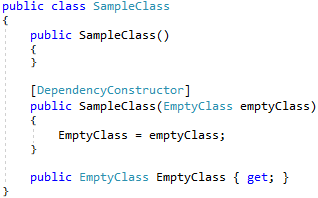
\includegraphics{DependencyConstructor.png}
	\end{raggedleft}
\end{figure}
Jest to główny i najbardziej popularny sposób wstrzykiwania zależności. Niektóre klasy mają kilka konstruktor i atrybut "DependencyConstructor" przydaje się wtedy do oznaczenia, który z nich ma zostać wybrany przy tworzeniu nowego obiektu. Jednakże nie zawsze jest on potrzebny. W większości przypadków klasy mają tylko jeden konstruktor, a także rozwiązania przemsysłowe mają logikę, która wybierze odpowiedni konstruktor (np. ten oznaczony atrybutem, albo ten co ma najwięcej parametrów, albo ten co ma najmniej parametrów).

\subsubsection{Wstrzykiwanie przez metodę}
\begin{figure}[h]
	\begin{raggedleft}
  		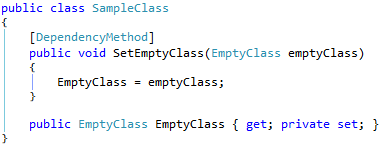
\includegraphics{DependencyMethod.png}
	\end{raggedleft}
\end{figure}
W przemysłowych rozwiązaniach to wstrzykiwanie z reguły odbywa się albo poprzez oznaczenie metody przez którą chcemy wstrzyknąć zaleźności odpowiednim atrybutem, albo przy rejestracji danej klasy definijumey przez jakie metody chcemy wstrzyknąć zależności.

\subsubsection{Wstrzykiwanie przez właściwość}
\begin{figure}[h]
	\begin{raggedleft}
  		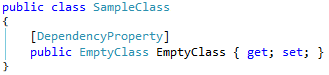
\includegraphics{DependencyProperty.png}
	\end{raggedleft}
\end{figure}
Tutaj podobnie jak dla wstrzykiwania przez metodę w przemysłowych rozwiązaniach to wstrzykiwanie z reguły odbywa się albo poprzez oznaczenie właściwoci przez którą chcemy wstrzyknąć zaleźności odpowiednim atrybutem, albo przy rejestracji danej klasy definijumey przez jakie właściwości chcemy wstrzyknąć zależności.


\clearpage
\subsection{Implementacje przemysłowe}
Na rynku jest wiele implementacji wstrzykiwania zależności. Przedstawię tutaj kilka najbardziej popularnych (według ilości pobrań z NuGet) oraz kilka najszybszych (według rankingu na stronie: http://www.palmmedia.de/Blog/2011/8/30/ioc-container-benchmark-performance-comparison). Dane zostały wzięte z dnia 21-02-2017. W nawiasie znajduje się wersja implementacji, która została użyta w testach (najnowsza na ten dzień).\\
\\
Najbardziej popularne:
\begin{itemize}
	\item Unity (4.0.1) - ponad 5.2 mln pobrań
	\item NInject (3.2.2) - ponad 4.0 mln pobrań
	\item Autofac (4.3.0) - ponad 3.7 mln pobrań
	\item StructureMap (4.4.3) - ponad 1.6 mln pobrań
	\item Windsor (3.4.0) - ponad 1.4 mln pobrań
\end{itemize}
Najszybsze:
\begin{itemize}
	\item Grace (5.1.0)
	\item DryIoc (2.10.1)
	\item LightInject (5.0.1)
	\item SimpleInjector (3.3.2)
\end{itemize}



\clearpage
\section{Implementacja}
Kod źródłowy programu jest dostępnym w repozytorium pod adresem:\\
\url{https://github.com/amularczyk/NiquIoC}\\
Znajduje się tam również kod programu, który posłużył do wykonania testów wydajnościowych, a także ta praca napisana w języku LateX i wszystkie obrazki.

\subsection{Środowisko pracy}
Prac oraz wszystkie testy powstały na komputerze z parametrami:
\begin{itemize}
	\item Intel Core i7-4720HQ (2.60GHz)
	\item 12 GB pamięci RAM
	\item Dysk SSD
\end{itemize}
Narzędzia użyte do stworzenia pracy i testów:
\begin{itemize}
	\item System operacyjny Windows 10 Pro
	\item .Net Framework w wersji 4.6.1
	\item Visual Studio 2017 Comunnity
	\item MSTest
	\item ReSharper
	\item dotCover
	\item Dia
\end{itemize}


\subsection{Wstęp}
Na początku chciałbym pokrótce opisać dwie rzeczy, które są istotne dla mojego rozwiązania. Pierwszą z nich jest Microsoft Intermediate Language, a drugą przestrzeń nazw Reflection.Emit.

\subsubsection{Microsoft Intermediate Language}
Microsoft Intermediate Language - MSIL (w skrócie IL) to język pośredni do którego kod C\# jest kompilowany. Język ten pozwala na komunikację między aplikacjami napisanymi na platformie .Net, a systemem operacyjnym. Jest on jądrem tej platformy.

\subsubsection{Reflection.Emit}
Przestrzeń nazw Reflection.Emit pozwala w języku C\# na stworzenie ciągu operacji w języku IL, a następnie zapamiętaniu ciągu tych operacji jako delegat. Za każdym razem, gdy ten delegat zostanie wywołany, to wykona się ciąg wczeniej zdefiniowanych operacji IL.


\subsection{Opis}
Aplikacja składa się z 1 projektu i 8 projektów na potrzeby testów. Rozwiązanie jest skomplikowana i aby mieć pewność, że działa w pełni dobrze zostało stworzone  ponad 1200 testów jednostkowych, a pokrycie kodu testami wynosi ponad 97\%.\\

W wykonanej implementacji został stworzony interfejs IConatiner, który definiuje operacje, jakie powinny się znaleźć w każdym kontenerze:
\begin{figure}[h]
	\begin{raggedleft}
  		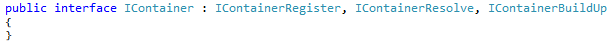
\includegraphics{IContainer.png}
	\end{raggedleft}
\end{figure}\\
Pierwsze cztery metody służą do rejestracji typów w kontenerze. Metoda piąta (Resolve) służy do tworzenia i zwracania obiektów wczeniej zarejestrowanych typów. Ostatnia metoda (BuildUp) do uzupełnienia istniejącej istancji obiektu z wykorzystaniem wstrzykiwania zależności przez metodę i właściwość - jest to metoda opcjonalna i nie każde przemysłowe rozwiązanie ją zawiera.\\
Poniżej znajduje się dokładniejszy opis każdej z metod.

\clearpage
\subsubsection{Register}
W pierwszej metodzie możemy zarejestrować zwykłe klasy. W drugiej interfejsy i klasy, które implementują dany interfejs lub klasy i klasy po nich dziedziczące. W trzeciej metodzie rejestrujemy klasę jako fabrykę obiektów - funkcję, która ma nam zwrócić pożądany obiekt. W czwartej natomiast możemy zarejestrować konkretną instancję danego typu.\\
W moim rozwiązaniu każdy typ może być zarejestrowany tylko raz - ponowna rejestracja tego samego typu nadpisuje istniejącą rejestrację.\\
Każda z tych czterech metod rejestracji zwraca interfejs IContainerMember, który umożliwia nam zarejestrowanie danego typu z określonym menadżerem czasu życia (czyli implementacją interfejsu IObjectLifetimeManager). Jest to po to, ponieważ dla różnych przypadków biznesowych możemy potrzebować, aby obiekt danego typu miał konretny czas życia. Interfejs IContainerMember wygląda następująco:
\begin{figure}[h]
	\begin{raggedleft}
  		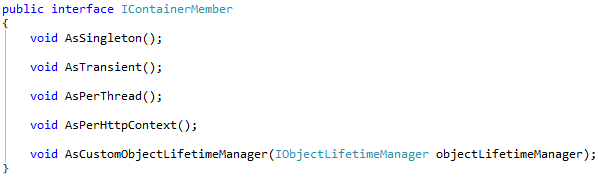
\includegraphics{IContainerMember.png}
	\end{raggedleft}
\end{figure}\\
Pierwsze cztery metody tego interfejsu to wbudowane implementacje interfejsu IObjectLifetimeManager. Piąta metoda dostarcza możliwoć podania przez użytkownika jego własnej implementacji tego interfejsu. W moim rozwiązaniu każdy typ domyślnie ma czas życia Transient.\\
\\
Wyjaśnienie rozdajów czasu życia:
\begin{itemize}
	\item Singleton - za każdym razem zwracany jest ten sam obiekt
	\item Transient - za każdym razem zwracany jest nowy obiekt
	\item PerThread - wewnątrz danego wątku zwracany jest ten sam obiekt, ale dla innego wątku zwracany jest nowy (inny) obiekt
	\item PerHttpContext - wewnątrz danego żądania Http zwracany jest ten sam obiekt, ale dla innego żądania zwracany jest nowy (inny) obiekt
\end{itemize}

\clearpage
Interfejs IObjectLifetimeManager prezentuje się tak:
\begin{figure}[h]
	\begin{raggedleft}
  		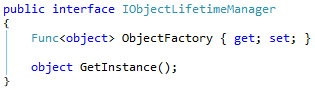
\includegraphics{IObjectLifetimeManager.png}
	\end{raggedleft}
\end{figure}\\
Właściwość ObjectFactory służy do ustawienia funkcji, która zwraca obiekt. Metoda GetInstance służy do pobrania obiektu.\\
W zależności od implementacji tego interfesju, to obiekt zwracany z metody GetInstance może być zawsze taki sam, zawsze różny albo taki sam tylko dla określonych sytuacji (np. taki sam dla tego samego wątku albo tego samego żądania http).

\subsubsection{Resolve}
Metoda piąta - Resolve, jest to główna operacja. Register można nazwać sercem kontenera, a Resolve mózgiem. Odpowiada ona za stworzenie i zwrócenie obiektu odpowiedniego typu.\\
W mojej pracy zaproponowałem dwa rozwiązania - PartialEmitFunction i FullEmitFunction, dlatego ta metoda jako parametr przyjmuje wartość enuma ResolveKind (dzięki temu w przyszłości może być ona w łatwy sposób rozszerzona o kolejne rozwiązania).

\subsubsection{BuildUp}
Szósta metoda to taki dodatek - gdy mamy stworzony obiekt, ale nie jest w pełni uzupełniony, wtedy możemy go zbudować (używająć odpowiedniej wartości z enuma ResolveKind). Z tą metodą są powiązane bezpośrednio dwa pojęcia - wstrzykiwanie przez metodę i wstrzykiwanie przez właściwość. Do tego celu w moim rozwiążaniu stworzyłem dwa atrybuty:
\begin{itemize}
	\item DependencyMethod (dla metod)
	\item DependencyProperty (dla właściwości)
\end{itemize}
Podczas operacji BuildUp wywoływane są wszystie metody i uzupełniane są wszystkie właściwości, które mają te atrybuty. Ta operacja jest również wykonywany podczas operacji Resolve.\\

Warto tutaj odnotować, że ze względu na szczegóły implementacyjne tylko jedno z moich rozwiązań wspiera operację BuildUp - jest to rozwiązanie PartialEmitFunction. W rozwiązaniu FullEmitFunction ta funckonalność nie została zaimplementowana. Jest to spowodowane skomplikowaniem tego rozwiązania i małą potrzebą biznesową używania tej operacji. Jednakże w przyszłości istnieje możliwość dodania implementacji tej funkcjonalności.\\

W aplikacji istnieje również atrybut DependencyConstrutor. Można go użyć przy definicji konstruktora danej klasy. Obiekt każdej klasy jest tworzony przy użyciu konstruktora. Klasa może mieć kilka konstruktorów. W moim rozwiązaniu stworzyłem logikę wyboru odpowiedniego konstruktora, przy pomocy którego ma zostać stworzony obiekt. Wygląda ona następująco:
\begin{itemize}
	\item Jeśli jest jeden konstruktor, to go wybierz.
	\item Jeśli jest kilka konstruktorów, to odpowiedni wybierz w poniższej kolejności:
	\begin{enumerate}
		\item Konstruktor z atrybutem DependencyConstrutor
		\item Konstruktor z największą liczbą parametrów
	\end{enumerate}
	\item Jeśli jest kilka konstrutkrów z atrybutem DependencyConstrutor albo nie ma żadnego konstruktora z tym atrybutem i jest kilka z największą liczbą parametrów, to rzuć wyjątek.
\end{itemize}


\subsection{Rozwiązanie}
Stworzenie nowego obiektu zajmuje czas. Gdy graf zależności dla jakiegoś typu jest bardzo rozbudowany, to stworzenie obiektu takiego typu zajmuje dużo czasu. Proces ten można podzielić na trzy etapy:
\begin{itemize}
	\item Uzyskanie informacji jakich typów obiekty są potrzebne do stworzenia danego obiektu.
	\item Stworzenie tych pomocnicznych obiektów.
	\item Stworzenie docelowego obiektu.
\end{itemize}
Gdy mamy rozbudowane grafy zależności, to często zdaża się, że niektóre typy się powtarzają. Zatem pewne informacje możemy uzyskać raz, a następnie je zapamiętać. Aby implementacja wzorca wstrzykiwania zależności działała wydajnie dla złożonych grafów zależności, należy jak najwięcej informacji przechowywać w pamięci podręcznej i należy to robić mądrze.\\
W mojej implementacji stworzyłem dwie strategie, które realizują te założenia. Pierwszy krok jest taki sam dla obu rozwiązań (uzyskanie informacji jakich typów obiekty są potrzebne do stworzenia danego obiektu), natomiast kolejne kroki już się różnią. W pierwszym rozwiązaniu, które nazwałem PartialEmitFunction całym process tworzenia nowego obiektu został rozbity na mniejsze części (docelowy obiekt jest tworzony po kawałku). Każda taka osobna część jest zapisywana w pamięci podręcznej. W drugim rozwiązaniu w pamięci podręcznej jest zapisana tylko jedna operacja. Zawiera ona listę wszystkich kroków, które są niezbędne do stworzenia docelowego obiektu. Więc finalnie docelowy obiekt jest tworzony przy pomocy jednej operacji (kroki drugi i trzeci są połączone). To rozwiązanie nazwałem FullEmitFunction.\\
W obu rozwiązaniach do zapamiętania kroków potrzebnych do stworzenia obiektu danego typu wykorzystałem operacje z przestrzeni nazw Reflection.Emit.

\subsubsection{Krok pierwszy}
Na początku algorytmu znajdujemy odpowiedni kontstruktor, przy pomocy którego ma zostać stworzony nowy obiekt. Jeśli robimy to poraz pierwszy dla danego typu, to informację o tym konstruktorze zapisujemy w pamięci podręcznej. Do tego celu została użyta struktura danych Dictionary, gdzie kluczem jest typ obiektu, a wartością obiekt klasy ContainerMember (w którym przechowujemy wszystkie zapamiętane informacje dla danego typu). Następnym krokiem, jest rekurencyjne wywołanie tej operacji dla wszystkich typów, których obiekty są niezbędne do stworzenia obiektu docelowego typu.\\
W tej operacji jest kilka wyjątków - są nimi typy zarejestrowane jako Instance albo FactoryObject. Dla pierwszego przypadku nie musimy uzyskiwać informacji o tym jak stworzyć obiekt takiego  typu, ponieważ mamy już taki obiekt stworzony i go po prostu wykorzystamy. Dla drugiego przypadku obiekt tworzony jest przy użyciu wcześniej zdefiniowanej przez użytkownika funkcji, której wywołanie spowoduje stworzenie obiektu oczekiwanego typu.
\clearpage
Klasa ContainerMember prezentuje się następująco:
\begin{figure}[h]
	\begin{raggedleft}
  		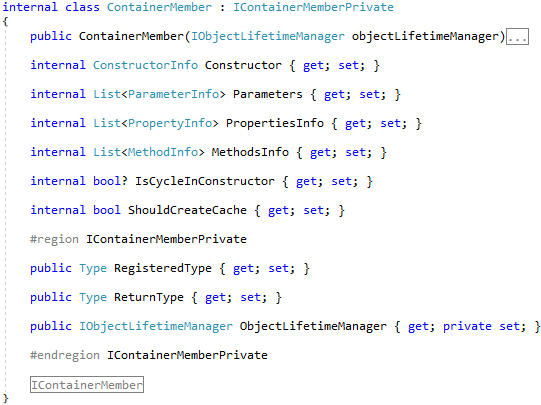
\includegraphics{ContainerMember.png}
	\end{raggedleft}
\end{figure}\\
Ta klasa przechowuje:
\begin{itemize}
	\item Informacje o konstruktor, przy pomocy którego należy utworzyć obiekt danego typu.
	\item Informacje o parametrach tego konstruktora.
	\item Informacje o właciwościach danego typu (na potrzeby operacji BuildUp).
	\item Informacje o metodach danego typu (na potrzeby operacji BuildUp).
	\item Czy występuję cykl w konstruktorze.
	\item Przy należy zapamiętać infrmacje dla danego typu (domyślnie tak, dla typóW zarejestrowanych jako Instance albo ObjectFactory - nie).
	\item Zarejestrowany typ (ta sama wartoć, co klucz ze słownika).
	\item Zwracany typ.
	\item Informacje o menadżerze cyklu życia.
\end{itemize}

\subsubsection{Rozwiązanie 1 - PartialEmitFunction}
Cały algorytm jest zawarty w metodzie Resolve. Sama ta metoda jest dość krótka, ale wywołuje ona kolejne metody (które już są dłuższe).\\
Docelowy obiekt jest tworzony przy pomocy funkcji. Na początku sprawdzamy, czy już wcześniej utworzyliśmy taką funkcję (jeśli tak, będzie on zapisany w klasie ContainerMember we właściwoci ObjectLifetimeManager). Wywołanie funkcji kończy działanie algorytmu. Jeśli funkcja nie została jeszcze wcześniej utworzona, to ją tworzymy.\\
Funkcja ta nie przyjmuje żadnych parametrów, a jej typem wynikowym jest obiekt. Ciało tej funkcji jest bardzo proste - po prostu ma ona wykonać metodę i zwrócić jej rezultat, którym jest nasz docelowy obiekt.
\begin{figure}[h]
	\begin{raggedleft}
  		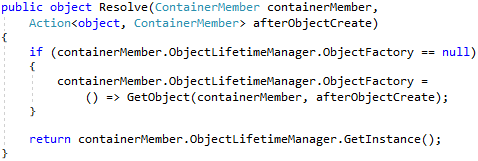
\includegraphics{PartialEmitFunction_Resolve.png}
	\end{raggedleft}
\end{figure}\\
Metoda GetObject jest trochę bardziej rozbudowana. Na początku pobieramy informacje o parametrach konstruktora danego typu. Następnie dla każdego z tych parametrów tworzomy obiekt (o docelowym typie) przy pomocy funkcji Resolve (opisanej wyżej). Korzystamy tutaj z rekurencji. Gdy już mamy stworzone obiekty dla każdego z parametrów konstruktora, to listę tych parametrów przekazujemy do metody CreateInstanceFunction, która zwróci nam instancję obiektu oczekiwanego typu. Na koniec wywołujemy callback afterObjectCreate i zwracamy nasz obiekt.
\begin{figure}[h]
	\begin{raggedleft}
  		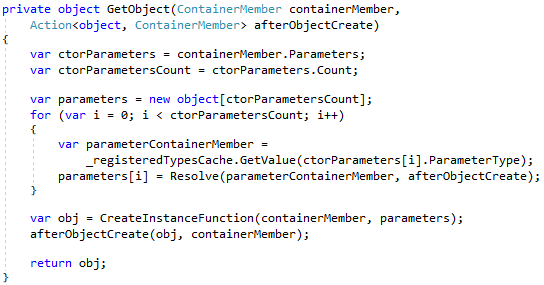
\includegraphics{PartialEmitFunction_GetObject.png}
	\end{raggedleft}
\end{figure}\\
Na początku metody CreateInstanceFunction sprawdzamy, czy mamy utworzoną funkcję, która umie zwrócić obiekt docelowego typu. Jeśli tak, to przy pomocy tej funkcji tworzymy obiekt  i go zwracamy. Ta funckja jako argument przyjmuje listę obiektów w kolejności zgodnej z listą parametrów konstruktora. Jeśli nie, to przy pomocy metody CreateObjectFunction tworzymy taką funkcję, a następnie zapisujemy ją w pamięci podręcznej (również w strukturze Dictionary, której kluczem jest type, a wartością jest funkcja).
\begin{figure}[h]
	\begin{raggedleft}
  		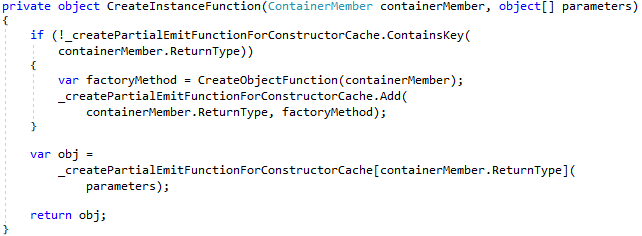
\includegraphics{PartialEmitFunction_CreateInstanceFunction.png}
	\end{raggedleft}
\end{figure}\\
CreateObjectFunction jest najbardziej zaawansowaną metodą w tym algorytmie. To w niej korzystamy z metod z przestrzeni nazw Reflection.Emit.\\
Na początku pobieramy informacje o konstruktorze. Następnie tworzymy DynamicMethod i z niej pobieramy ILGenerator. W nim będziemy przechowywać listę kroków niezbędnych do utworzenia docelowego obiektu.\\
Dla każdego z parametrów konstruktora wykonujemy następujące operacje:
\begin{enumerate}
	\item Dodaj do listy kroków operację, która umieści na szczycie stosu pierwszy parametr (będzie nim lista obiektów zgodna z parametrami konstruktora).
	\item Dodaj do listy kroków operację, która umieści na szczycie stosu indeks parametru (który to jest parametr z kolei).
	\item Dodaj do listy kroków operację, która zdejmie ze szczytu stosu listę i indeks, a umieści na jego szczycie element znajdujący się pod danym indeksem na liście.
	\item Pobieramy typ parametru.
	\item Dodaj do listy kroków operację, która zrzutuje obiekt ze szczytu stosu na odpowiedni typ.
\end{enumerate}
Po wykonaniu kroków z listy na stosie będziemy mieli wszystkie obiekty, które są wymagane przez konstruktor do utworzenia danego typu. Teraz więc do listy kroków dodajemy operację, która stworzy obiekty przy pomocy danego konstruktora i umieści go na szczycie stosu. Na koniec dodajemy krok, który zwróci nam obiekt ze szczytu stosu.\\
Wszystkie kroki niezbędne do stworzenia nowego elementu są zapisane w zmiennej typu DynamicMethod. Jako ostatnią operację w metodzie CreateObjectFunction, ze zmiennej typu DynamicMethod, tworzymy i zwracamy delegata, który jako parametr będzie przyjmował tablicę obiektów (nasza lista obiektów zgodna z parametrami konstruktora), a zwracał obiekt (nasz docelowy obiekt).
\begin{figure}[h]
	\begin{raggedleft}
  		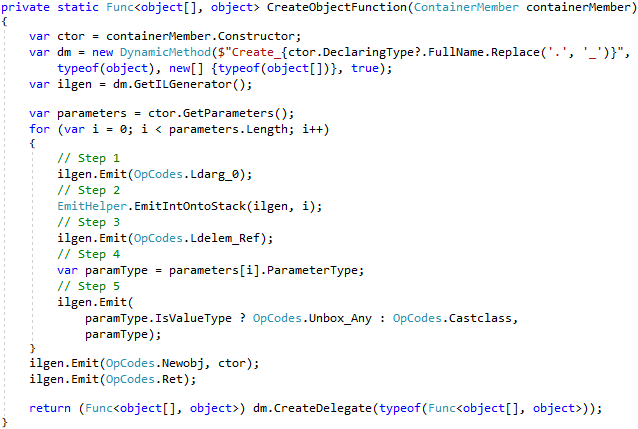
\includegraphics{PartialEmitFunction_CreateObjectFunction.png}
	\end{raggedleft}
\end{figure}

\clearpage
\subsubsection{Rozwiązanie 2 - FullEmitFunction}
Tutaj podobnie jak dla PartialEmitFunction cały algorytm zawarty jest w metodzie Resolve. Wygląda ona identycznie jak w rozwiązaniu 1 - docelowy obiekt jest tworzony przy pomocy funkcji, która woła w sobię metodę GetObject. Jeśli funkcji nie ma w zapisanej w pamięci, to ją tworzymy i zapisuje. Na końcu ją wywołujemy.
\begin{figure}[h]
	\begin{raggedleft}
  		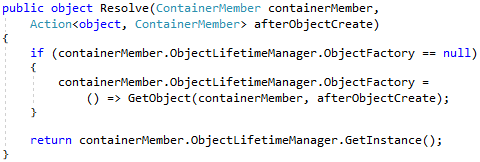
\includegraphics{FullEmitFunction_Resolve.png}
	\end{raggedleft}
\end{figure}\\
Metoda GetObject wygląda trochę inaczej. Nie pobieramy tutaj żadnych dodatkowych informacji, tylko od razu wywołujemy metodę CreateInstanceFunction, która zwróci nam instancję obiektu oczekiwanego typu. Na koniec również wywołujemy callback afterObjectCreate i zwracamy nasz obiekt.
\begin{figure}[h]
	\begin{raggedleft}
  		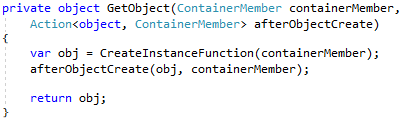
\includegraphics{FullEmitFunction_GetObject.png}
	\end{raggedleft}
\end{figure}\\
CreateInstanceFunction ma jeden dodatkowy krok względem rozwiązania 1. Na początku również sprawdzamy, czy mamy utworzoną funkcję, która umie zwrócić obiekt docelowego typu. Jeśli nie, to przy pomocy metody CreateObjectFunction tworzymy taką funkcję, a następnie zapisujemy ją w pamięci podręcznej (również w strukturze Dictionary, której kluczem jest type, a wartością jest typ pomocniczy FullEmitFunctionResult, który ma tylko jedną właściwość - Result typu funkcja). Następnym krokiem jest zwalidowanie zapisanych danych dla typów przy pomocy metody ValidateTypesCache. Na końcu funkcji tworzymy obiekt  i go zwracamy. Tutaj funckja jako argument przyjmuje dwa słowniki. Pierwszy zawiera informacje o typie (kluczem jest typ, a wartością obiekt ContainerMember), a drugi informacje o indeksie typu (kluczem jest liczba oznaczając hasz danego typu, a wartością typ).\\
Najpierw opiszę metodę ValidateTypesCache, ponieważ nie wywołuje ona w sobie żadnych innych metod.
\begin{figure}[h]
	\begin{raggedleft}
  		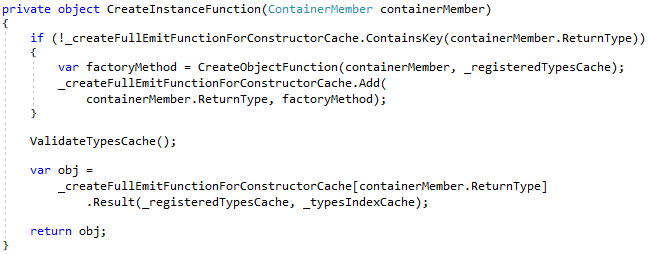
\includegraphics{FullEmitFunction_CreateInstanceFunction.png}
	\end{raggedleft}
\end{figure}\\
W pierwszym kroku metody ValidateTypesCache sprawdzamy, czy od ostatniego zapisywania danych o typach w pamięci podręcznej jakiś typ został zarejestorwany w kontenerze (lub czy jest to pierwsze zapisanie tych danych). Jeśli tak, to tworzymy z zarejestrowanych typów tworzymy słownik, w którym kluczem jest hasz typu, a wartością typ. Potem aktualizujemy liczbę aktualnie zarejestrowanych typów.
\begin{figure}[h]
	\begin{raggedleft}
  		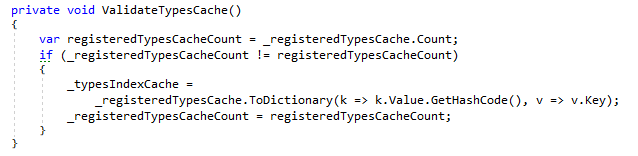
\includegraphics{FullEmitFunction_ValidateTypesCache.png}
	\end{raggedleft}
\end{figure}\\
Metoda CreateObjectFunction jest dużo bardziej rozbudowana niż w rozwiązaniu 1. W niej również korzystamy z metod z przestrzeni nazw Reflection.Emit.\\
Na początku tworzymy DynamicMethod i z niej pobieramy ILGenerator, w którym będziemy przechowywać listę kroków niezbędnych do utworzenia docelowego obiektu.\\
Dla każdego z parametrów konstruktora wywołujemy metodę CreateObjectFunctionPrivate, która uzupełni listę kroków o tworzenie pośrednich obiektów. To w tym miejscu jest główna różnica między oboma rozwiązaniami - w pierwszym rozwiązaniu w liście kroków nie przejmowaliśmy się utworzeniem pośrednich obiektów, ponieważ przychodziły one jako parametr. W tym rozwiązaniu lista kroków będzie również zawierać kroki do utworzenia wszystkich obiektów pośrednich (obiektów wymaganych przez konstruktory).\\
Dalsze operacje są takie same jak w rozwiązaniu 1 - do listy kroków dodajemy operację, która stworzy obiekty przy pomocy danego konstruktora i umieści go na szczycie stosu, a następnie dodajemy operację, który zwróci nam obiekt ze szczytu stosu.\\
Na końcu ze zmiennej typu DynamicMethod tworzymy delegata i go zwracamy. Delegat będzie przyjmował dwa parametry - oba typu Dictionaty. Jeden z informacjami o type, a drugi z informacjiami o indeksie typu.
\begin{figure}[h]
	\begin{raggedleft}
  		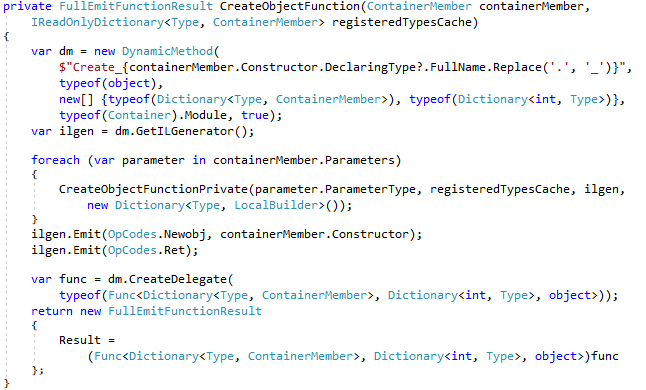
\includegraphics{FullEmitFunction_CreateObjectFunction.png}
	\end{raggedleft}
\end{figure}\\
W metodzie CreateObjectFunctionPrivate mamy trzy przypadki. W pierwszych dwóch przypadkach pomijamy obiekty, które zostały zarejestrowane jako Instance albo FactoryObject (określa to parametr ShouldCreateCache z obiektu typu ContainerMember).
\begin{figure}[h]
	\begin{raggedleft}
  		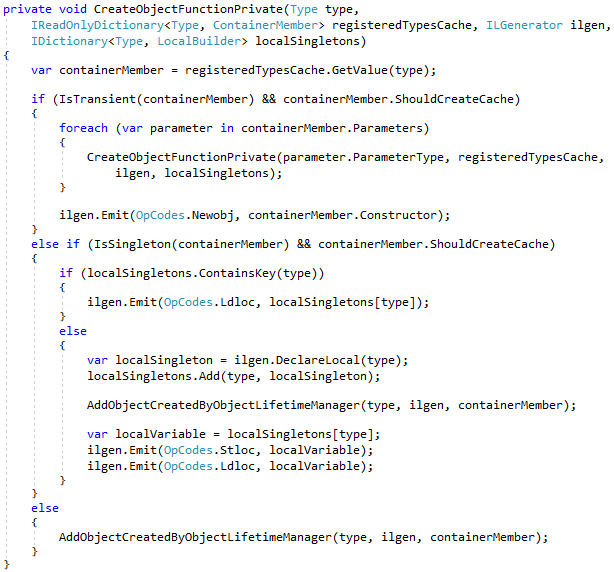
\includegraphics{FullEmitFunction_CreateObjectFunctionPrivate.png}
	\end{raggedleft}
\end{figure}\\
Pierwszy przypadek, to gdy typu jest Transient (obiekt został zarejestrowany jako Transient).\\
Wtedy dla każdego z parametrów konstruktora wywołujemy rekurencyjnie tę metodę (CreateObjectFunctionPrivate), a na koniec do listy kroków dodajemy operację, która stworzy obiekty przy pomocy danego konstruktora i umieści go na szczycie stosu.
\begin{figure}[h]
	\begin{raggedleft}
  		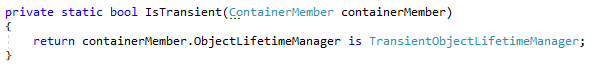
\includegraphics{FullEmitFunction_IsTransient.png}
	\end{raggedleft}
\end{figure}\\
W drugim przypadeku typ musi być singletonem (został on zarejestrowany jako Singleton, PerThread lub PerHttpContext).\\
Na początku sprawdzamy czy już wcześniej natrafiliśmy na ten typ. Jeśli tak, to z pamięci podręcznej pobieramy zmienną lokalną dla danego typu, a następnie do listy kroków dodajemy operację, która doda na szczyt stosu obiekt z tej zmiennej. Jeśli nie, to najpierw tworzymy nową zmienną lokalną dla danego typu i zapisuje ją w pamięci podręcznej (wykorzystujemy do tego słownik, gdzie kluczem jest typ, a wartością obiekt typu LocalBuilder). Następnie wywołujemy metodę AddObjectCreatedByObjectLifetimeManager. Na końcu dodajemy dwie operacje. Pierwsza z nich zdejmie obiekt ze szczytu stosu i zapisze go w zmiennej lokalnej, a druga umieści na szczycie stosu obiekt z tej zmiennej lokalnej. Jest to po to, ponieważ na szczycie stosu chcemy mieć dany obiekt, ale również chcemy zapamiętać sobie dany obiekt, aby nie trzeba było go tworzyć, jeśli będzie potrzebny poraz drugi (obiekt jest singletonem, więc za każdym razem będziemy chcieli mieć ten sam obiekt - w kontekście tworzenia danego typu, czyli jednej operacji Resolve).
\begin{figure}[h]
	\begin{raggedleft}
  		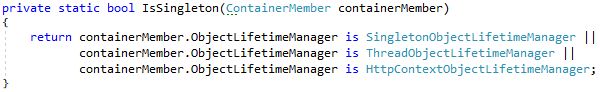
\includegraphics{FullEmitFunction_IsSingleton.png}
	\end{raggedleft}
\end{figure}\\
Metoda AddObjectCreatedByObjectLifetimeManager, za wyjątkiem pierwszej operacji jaką jest stworzenie zmiennej lokalnej typu Type, zawiera jedynie operacje, które dodają kolejne kroki do listy kroków:
\begin{enumerate}
	\item Dodaj do listy kroków operację, która umieści na szczycie stosu drugi parametr (będzie nim słownik z indeksami typów).
	\item Dodaj do listy kroków operację, która umieści na szczycie stosu hasz danego typu.
	\item Dodaj do listy kroków operację, która pobierze ze szczytu stosu słownik i indeks, a umieści na jego szczycie element znajdujący się pod danym kluczem w słowniku.
	\item Dodaj do listy kroków operację, która zdejmie obiekt ze szczytu stosu i zapisze go w zmiennej lokalnej.
	\item Dodaj do listy kroków operację, która umieści na szczycie stosu pierwszy parametr (będzie nim słownik z informacjami o typach).
	\item Dodaj do listy kroków operację, która umieści na szczycie stosu obiekt ze zmiennej lokalnej.
	\item Dodaj do listy kroków operację, która zdejmie ze szczytu stosu słownik i typ, a umieści na jego szczycie element znajdujący się pod danym kluczem w słowniku.
	\item Dodaj do listy kroków operację, która zdejmie obiekt ze szczytu stosu (będzie to obiekt typu ContainerMember), wywoła na nim metodę, która zwróci menadżer czasu życia obiektu i na szczycie stosu umieści rezultat tej metody.
	\item Dodaj do listy kroków operację, która zdejmie obiekt ze szczytu stosu (będzie to obiekt typu IObjectLifeTimeManager), wywoła na nim metodę, która zwróci instancję obiektu i na szczycie stosu umieści rezultat tej metody.
	\item Dodaj do listy kroków operację, która zrzutuje obiekt ze szczytu stosu na odpowiedni typ.
\end{enumerate}
Po wykonaniu tych 10 operacji na szczycie stosu znajdzie się obiekt danego typu utworzony przy pomocy menadżera czasu życia.
\begin{figure}[h]
	\begin{raggedleft}
  		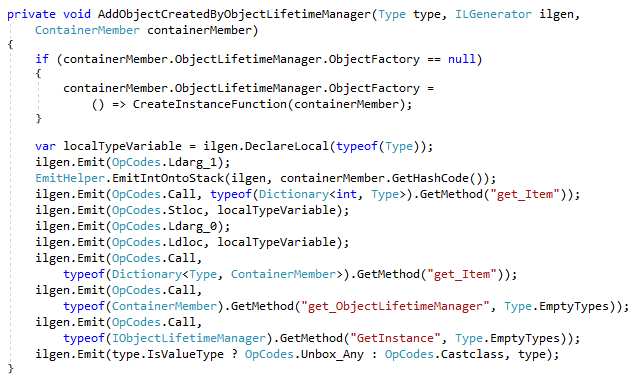
\includegraphics{FullEmitFunction_AddObjectCreatedByObjectLifetimeManager.png}
	\end{raggedleft}
\end{figure}\\
Trzeci przypadek zachodzi gdy typ został zarejestrowany jako Instance, FactoryObject lub przy pomocy własnego menadżera czasu życia (implementacji interfejsu IObjectLifetimeManager).\\
W tej sytuacji wywołujemy po prostu metodę AddObjectCreatedByObjectLifetimeManager.



\clearpage
\section{Testy wydajnościowe}
Do przeprowadzania testów wydajnościowych stworzyłem osobną aplikację w której utworzyłem 4 przypadki testowe:
\begin{itemize}
	\item Przypadek testowy A,
	\item Przypadek testowy B,
	\item Przypadek testowy C,
	\item Przypadek testowy D.
\end{itemize}
Dla każdego z przypadków sprawdzany jest czas wykoniania operacji "Resolve" dla różnych rodzajów rejestracji (operacji Register).Testy zostały wykonane dla następujących wariantów rejestracji:
\begin{itemize}
	\item Register as Singleton,
	\item Register as Transient,
	\item Register as TransientSingleton,
	\item Register as PerThread (dla niektórych przemysłowych rozwiązań - PerScope),
	\item {\color{red}Register as FactoryMethod.}
\end{itemize}
Każdy z testów dla każdego rozwiązania był uruchamiany w osobnym procesie. Każdy test był uruchamiany 100 razy, a w wynikach zostały przedstawione następujące czasy: minimalny, maksymalny i średni.

\subsubsection{Register as Singleton}
Każdy typ jest zarejestrowany jako "Singleton", czyli obiekt jest tworzony raz, a następnie cały czas zwracany.

\subsubsection{Register as Transient}
Każdy typ jest zarejestrowany jako "Transient", czyli za każdym razem jest tworzony nowy obiekt.

\subsubsection{Register as TransientSingleton}
Każdy typ jest zarejestrowany jako "Transient" za wyjątkiem typów, które maja konstruktor bezparametrowy - są one zarejestrowane jako "Singleton".

\subsubsection{Register as PerThread}
Każdy typ jest zarejestrowany jako "PerThread", czyli obiekt jest tworzony raz dla każdego wątku, a następnie w obrębie tego wątku cały czas zwracany.

\subsubsection{Register as FactoryMethod}
{\color{red}Typ główny jest zarejestrowany jako "FactoryMethod", czyli jako funkcja, która zwraca nam obiekt danego typu.}

\subsection{Przypadek testowy A}
\subsubsection{Opis}
W tym teście mamy zdefiniowanych 11 typów. Każdy z nich przymuje w konstruktorze o jeden parametr mniej niż typ poprzedni (czyli przyjmują one kolejno od 10 do 0 parametrów w konstruktorze). Typem głównym, a zarazem typem o największej liczbie parametrów, jest typ "TestA". Przyjmuje on w konstruktorze 10 parametrów następujących typów: "TestA0", "TestA1", "TestA2", "TestA3", "TestA4", "TestA5", "TestA6", "TestA7", "TestA8", "TestA9". Każdy z tych 10 typów w konstruktorze przyjmuje tyle parametrów, jaki ma numerek w nazwie (czyli obiekt typu "TestA0" ma konstruktore bezparametrowy, obiekt typy "TestA1" ma konstuktor z jednym parametrem; i tak dalej aż do typu "TestA9", który ma konstruktor z dziewięcioma parametrami). Wszystkie typy jako parametry w konstruktorze przyjmuje obiekty typów z niższymi numerkami (czyli obiekt typu "TestA1" w konstruktorze przyjmuje obiekt typu "TestA0", obiekt typu "TestA2" przymuje w konstruktorze obiekty typóW "TestA0" i "TestA1";  i tak dalej aż do typu "TestA9", który w konstruktorze przyjmuje obiekty z typami od "TestA0" do "TestA8"). Graf zależności poszczególnych typów został przedstawiony na Rys. \ref{fig:testA}.
\begin{figure}[h]
	\begin{center}
  		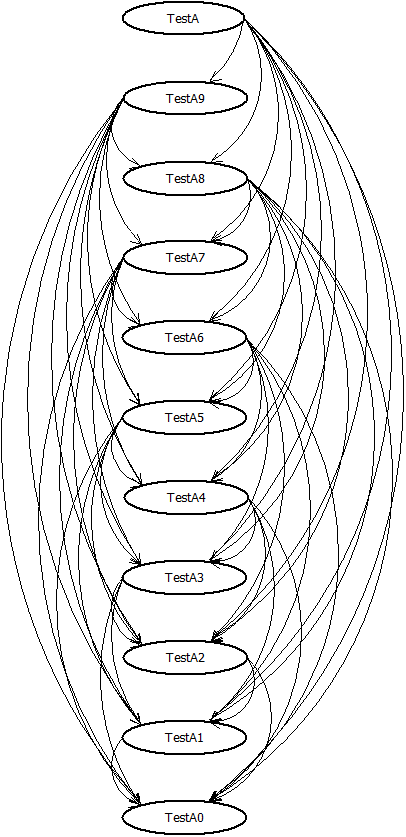
\includegraphics[height=12cm]{TestA.png}
  		\caption{Graf zależności dla testu A.}
  		\label{fig:testA}
	\end{center}
\end{figure}\\

Łatwo wywnioskować, że tworząc obiekty poszczególnych typów ilość tworzonych obiektów rośnie dwukrotnie:
\begin{itemize}
	\item TestA0 - 1 obiekt,
	\item TestA1 - 2 obiekty (obiekt typu TestA1 i obiekt typu TestA0),
	\item TestA2 - 4 obiekty (obiekt typu TestA2, obiekt typu TestA1 - 2 obiekty, obiekt typu TestA0 - 1 obiekt),
	\item TestA3 - 8 obiektów (obiekt typu TestA3, obiekt typu TestA2 - 4 obiekty, obiekt typu TestA1 - 2 obiekty, obiekt typu TestA0 - 1 obiekt),
	\item TestA4 - 16 obiektów,
	\item TestA5 - 32 obiektów,
	\item TestA6 - 64 obiektów,
	\item TestA7 - 128 obiektów,
	\item TestA8 - 256 obiektów,
	\item TestA9 - 512 obiektów,
	\item TestA - 1 024 obiektów.
\end{itemize}
Zatem tworząc nasz główny obiekt typu TestA, tworzymy: 1 obiekt typu TestA, 1 obiekt typu TestA9, 2 obiekty typu TestA8, 4 obiekty typu TestA7, 8 obiektów typu TestA6, 16 obiektów typu TestA5, 32 obiektów typu TestA4, 64 obiektów typu TestA3, 128 obiektów typu TestA2, 256 obiektów typu TestA1 i 512 obiektów typu TestA0 - co w sumie daje 1024 obiekty.

\subsubsection{Wyniki dla Singleton}
\begin{center}
\begin{small}
	\begin{tabular}{ | l | r r r | r r r | r r r | r r r | }
    		\hline
Ilość & & 1 & & & 10 & & & 100 & & & 1000 & \\ \hline
 & min & max & avg & min & max & avg & min & max & avg & min & max & avg \\ \hline
Autofac & 0 & 0 & 0 & 0 & 0 & 0 & 0 & 0 & 0 & 0 & 0 & 0 \\ \hline
DryIoc & 2 & 2 & 2 & 2 & 2 & 2 & 2 & 2 & 2 & 2 & 2 & 2 \\ \hline
Grace & 2 & 2 & 2 & 2 & 2 & 2 & 2 & 2 & 2 & 2 & 3 & 2 \\ \hline
LightInject & 2 & 2 & 2 & 2 & 2 & 2 & 2 & 2 & 2 & 2 & 2 & 2 \\ \hline
Ninject & 3 & 3 & 3 & 3 & 3 & 3 & 3 & 3 & 3 & 6 & 7 & 6 \\ \hline
NiquIoCPartial & 1 & 1 & 1 & 1 & 1 & 1 & 1 & 1 & 1 & 1 & 1 & 1 \\ \hline
NiquIoCFull & 2 & 2 & 2 & 2 & 2 & 2 & 2 & 3 & 2 & 2 & 2 & 2 \\ \hline
SimpleInjector & 2 & 2 & 2 & 2 & 2 & 2 & 2 & 2 & 2 & 2 & 2 & 2 \\ \hline
StructureMap & 9 & 10 & 9 & 9 & 10 & 9 & 9 & 10 & 9 & 10 & 11 & 10 \\ \hline
Unity & 7 & 8 & 7 & 7 & 8 & 7 & 7 & 8 & 7 & 8 & 8 & 8 \\ \hline
Windsor & 0 & 0 & 0 & 0 & 0 & 0 & 0 & 0 & 0 & 0 & 0 & 0 \\ \hline
  	\end{tabular}
\end{small}
\end{center}
Dla tego testu najlepiej poradziły sobie dwa z najpopularniejszych rozwiązania - Aurofac i Windsor. Rozwiązanie NiquIoCPartial uplasowało się na 3 miejscu. Najsłabiej poradził sobie pozostałe najpopularniejsze rozwiązania: Ninject, Unity oraz StructureMap. Reszta rozwiązań miała zbliżone czasy - dwukrotnie większe niż NiquIoCPartial i trzykrotnie mniejsze niż Ninject.

\subsubsection{Wyniki dla Transient}
\begin{center}
\begin{small}
	\begin{tabular}{ | l | r r r | r r r | r r r | r r r | }
    		\hline
Ilość & & 1 & & & 10 & & & 100 & & & 1000 & \\ \hline
 & min & max & avg & min & max & avg & min & max & avg & min & max & avg \\ \hline
Autofac & 0 & 0 & 0 & 6 & 7 & 6 & 58 & 63 & 59 & 584 & 609 & 587 \\ \hline
DryIoc & 14 & 14 & 14 & 14 & 15 & 15 & 16 & 16 & 16 & 29 & 30 & 29 \\ \hline
Grace & 15 & 16 & 15 & 15 & 16 & 16 & 18 & 19 & 18 & 37 & 38 & 37 \\ \hline
LightInject & 10 & 10 & 10 & 10 & 10 & 10 & 11 & 12 & 11 & 19 & 20 & 19 \\ \hline
Ninject & 10 & 12 & 11 & 88 & 95 & 90 & 864 & 1035 & 882 & 8745 & 9610 & 8934 \\ \hline
NiquIoCPartial & 1 & 1 & 1 & 3 & 3 & 3 & 19 & 22 & 19 & 171 & 198 & 173 \\ \hline
NiquIoCFull & 8 & 9 & 8 & 8 & 9 & 8 & 9 & 10 & 9 & 18 & 19 & 18 \\ \hline
SimpleInjector & 13 & 14 & 13 & 13 & 14 & 14 & 15 & 15 & 15 & 28 & 30 & 29 \\ \hline
StructureMap & 10 & 10 & 10 & 13 & 14 & 14 & 53 & 55 & 54 & 414 & 457 & 417 \\ \hline
Unity & 8 & 9 & 8 & 16 & 17 & 16 & 88 & 91 & 88 & 803 & 961 & 813 \\ \hline
Windsor & 1 & 2 & 1 & 16 & 21 & 16 & 152 & 192 & 155 & 1511 & 1799 & 1529 \\ \hline
  	\end{tabular}
\end{small}
\end{center}
W tym teście jest już spora rozbieżność czasów. Gdy mamy tylko 1 operację najlepiej radzi sobie Autofac, a zaraz za nim NiquIoCPartial i Windsor. Najsłabiej natomiast SimplyInjector, DryIoc i Grace. Pozostałe rozwiązania wypadły przeciętnie i bliżej im było do czasów najgorszych, niż najlepszych.\\
Dla 10 operacji sytuacja zaczyna się lekko zmieniać. Tym razem znacząco najlepiej radzi sobie NiquIoCPartial - ponad dwa razy lepiej niż drugi Autofac. Kolejne miejsca należą do NiquIoCFull i LightInject. Pozostałe rozwiązania miały podobne, trochę słabsze czasy. Wyjątkiem jest jedynie Ninject, który poradził sobie najgorzej i jego czas jest ponad 5 razy większy niż dla rozwiązania z przedostatnim czasem (Windsor).\\
Przy 100 operacji na prowadzenie wysuneły się mniej popularne rozwiązania. Na pierwszym miejscu jest NiquIoCFull, a kolejne miejsca to LightInject i SimpleInjector. DryIoc, Grace oraz NiquIoCPartial wypadły akceptowalnie - poradziły sobie trochę gorzej niż trzeci SimpleInjector. Do grona najsłabszych (Unity, Windsor, Ninject) w tym przypadku dołączył również Autofac, który z drugiego miejsca spadł na ósme. StructureMap miał czasy tylko trochę lepszy niż Autofac.\\
Natomiast dla 1000 operacji od czołówki oddalił się NiquIoCPartial. Na pierwszym miejscu wciąż pozostaje NiquIoCFull, a zaraz za nim LightInject i SimpleInjector. DryIoc i Grace wciąż tochę słabiej, ale nadal zadowalająco. Pozostałe rozwiązania mają czasy od kilku do kilkunastu razy gorsze niż reszta. Bez cienia wątpliwości najgorzej wypadł Ninjec.\\
Warto tutaj zaznaczyć, że wraz ze wzrostem operacji najmniejszy wzorst czasów miały rozwiązania: LightInject, NiquIoCFull, SimpleInjector, DryIoc oraz Grace.

\subsubsection{Wyniki dla TransientSingleton}
\begin{center}
\begin{small}
	\begin{tabular}{ | l | r r r | r r r | r r r | r r r | }
    		\hline
Ilość & & 1 & & & 10 & & & 100 & & & 1000 & \\ \hline
 & min & max & avg & min & max & avg & min & max & avg & min & max & avg \\ \hline
Autofac & 0 & 0 & 0 & 6 & 7 & 6 & 53 & 62 & 54 & 531 & 561 & 535 \\ \hline
DryIoc & 18 & 19 & 18 & 19 & 19 & 19 & 20 & 21 & 20 & 31 & 32 & 32 \\ \hline
Grace & 9 & 10 & 10 & 10 & 10 & 10 & 10 & 11 & 11 & 18 & 19 & 18 \\ \hline
LightInject & 14 & 15 & 14 & 14 & 14 & 14 & 14 & 15 & 15 & 20 & 21 & 20 \\ \hline
Ninject & 9 & 10 & 10 & 65 & 82 & 67 & 626 & 743 & 641 & 6297 & 7218 & 6463 \\ \hline
NiquIoCPartial & 1 & 1 & 1 & 2 & 3 & 2 & 14 & 15 & 14 & 120 & 123 & 121 \\ \hline
NiquIoCFull & 5 & 6 & 5 & 5 & 6 & 5 & 6 & 6 & 6 & 10 & 12 & 11 \\ \hline
SimpleInjector & 9 & 9 & 9 & 9 & 10 & 9 & 10 & 11 & 10 & 17 & 19 & 17 \\ \hline
StructureMap & 9 & 10 & 10 & 12 & 12 & 12 & 35 & 40 & 36 & 252 & 306 & 256 \\ \hline
Unity & 8 & 9 & 8 & 14 & 15 & 14 & 73 & 82 & 74 & 659 & 753 & 663 \\ \hline
Windsor & 1 & 2 & 1 & 12 & 14 & 12 & 117 & 140 & 119 & 1161 & 1302 & 1177 \\ \hline
  	\end{tabular}
\end{small}
\end{center}
Przy tym teście dla 1 operacji również najlepiej poradziły sobie Autofac, NiquIoCPartial i Windsor. Trochę gorzej NiquIoCFull. Czasy dla Unity, SimpleInjector, Grace, StructureMap i Ninject są zbliżone, jednak duże. Najgorzej wypadły natomiast LightInject i DryIoc.\\
Gdy mamy 10 operacji na drugie miejsce wskoczył NiquIoCFull. Na pierwsze przesunął się NiquIoCPartial, a Autofac spadł na trzecie. Kolejne miejsce zajmują SimpleInjector i Grace. Trochę gorzej poradził sobie StrutureMap. Zaraz za nim jest Windsor, który z podium spadł na 7 miejsce. Kolejne miejsca to LightInject i Unity. DryIoc nadal słabo, jednakże wzrostu czasu był nieduży. Ostatnie miejsce zajął Ninject.\\
Dla 100 operacji na pierwszym miejscu znalazł się NiquIoCFull. Na podium znaleźli się jeszcze SimpleInjector i Grace. NiquIoCPartial spadł poza podium, a tuż za nim jest LightInject. DryIoc nadal z niedużym wzrostem czasu i tym razem jego wynik jest już akceptowalny. Pozostałe rozwiążań bardzo słabo. Kolejne miejsca to StructureMap oraz Autofac, a ranking zamykają Unity, Windsor i Ninject.\\
Test dla 1000 operacji nie spowodował żadnych zmiań w rankingu. Jedynie różnica czasów pomiędzy pierwszą 5, a pozostały miejscami znacząco się zwiększyła. Dla pierwszej piątki czasy zwrosły około dwukrotkie, a dla pozostały miejsc ponad siedmiokrotnie.

\subsubsection{Wyniki dla PerThread}
\begin{center}
\begin{small}
	\begin{tabular}{ | l | r r r | r r r | r r r | r r r | }
    		\hline
Ilość & & 1 & & & 10 & & & 100 & & & 1000 & \\ \hline
 & min & max & avg & min & max & avg & min & max & avg & min & max & avg \\ \hline
Autofac & 0 & 0 & 0 & 0 & 0 & 0 & 0 & 0 & 0 & 0 & 0 & 0 \\ \hline
DryIoc & 71 & 73 & 71 & 71 & 72 & 71 & 71 & 73 & 72 & 72 & 74 & 72 \\ \hline
Grace & 4 & 4 & 4 & 4 & 4 & 4 & 4 & 4 & 4 & 4 & 4 & 4 \\ \hline
LightInject & 50 & 53 & 50 & 50 & 51 & 50 & 50 & 54 & 51 & 50 & 52 & 51 \\ \hline
Ninject & 3 & 3 & 3 & 3 & 3 & 3 & 3 & 3 & 3 & 6 & 7 & 6 \\ \hline
NiquIoCPartial & 1 & 1 & 1 & 1 & 1 & 1 & 1 & 1 & 1 & 1 & 1 & 1 \\ \hline
NiquIoCFull & 2 & 2 & 2 & 2 & 2 & 2 & 2 & 3 & 2 & 2 & 2 & 2 \\ \hline
SimpleInjector & 7 & 8 & 8 & 8 & 8 & 8 & 8 & 8 & 8 & 8 & 8 & 8 \\ \hline
StructureMap & 9 & 10 & 9 & 9 & 10 & 9 & 9 & 10 & 9 & 10 & 10 & 10 \\ \hline
Unity & 7 & 8 & 7 & 7 & 8 & 7 & 7 & 8 & 7 & 8 & 9 & 8 \\ \hline
Windsor & 0 & 0 & 0 & 0 & 0 & 0 & 0 & 0 & 0 & 0 & 0 & 0 \\ \hline
  	\end{tabular}
\end{small}
\end{center}
Czasy dla tego przypadku powinny być zbliżone do czasów dla przypadku Singleton, ponieważ wszystko było uruchamiane w jednym wątku. Niestety część rozwiązań sobie z tym nie poradziła.\\
Wyniki zbliżone posiadają: Autofac, Grace, Ninject, NiquIoCPartial, NiquIoCFull, StructureMap, Unity i Windsor. Natomiast dla SimpleInjector, LightInject i DryIoC czasy są od kilku do nawet kilkudziesięciu razy większe.\\
Jeśli chodzi o najlepsze rozwiązania, to wyglądają one tak samo jak dla Singleton. Pierwsze trzy miejsca to Aurofac, Windsor i NiquIoCPartial. Najsłabiej poradziły sobie LightInject i DryIoc. Tuż za czołówką znalazły się: NiquIoCFull, Grace i Ninject. Dla 1, 10 i 100 operacji wyżej uplasował się Ninject, a dla 1000 Grace. W drugiej połowie rankingu miejsca przypadły: SimpleInjector, Unity i StructureMap. Unity poradziło sobie gorzej niż SimpleInjector dla 1000 operacji, ale lepiej w pozostałych trzech przypadkach.


\subsection{Przypadek testowy B}
\subsubsection{Opis}
Ten test jest bardzo podobny do przypadku testowego A, tylko dochodzi nam 1 dodatkowy poziom, który wygląda trochę inaczej. W głównym obiekcie "TestB" konstruktor przyjmuje 3 parametry następujących typów: "TestBa10", "TestBb10", "TestBc10". Każdy z tych 3 typów odpowiada typowi "TestA", więc przyjmuje on w konstruktorze 10 parametrów. Dla "TestBa10" są to parametry typów od "TestBa0" do "TestBa9", dla "TestBb10" są to parametry typów od "TestBb0" do "TestBb9", a dla "TestBc10" są to parametry typów od "TestBc0" do "TestBc9". Zależności tych typów wyglądają tak samo, jak dla typów z przypadku testowego A - rys. \ref{fig:testB} przedstawia te zależności.
\begin{figure}[h]
	\begin{center}
  		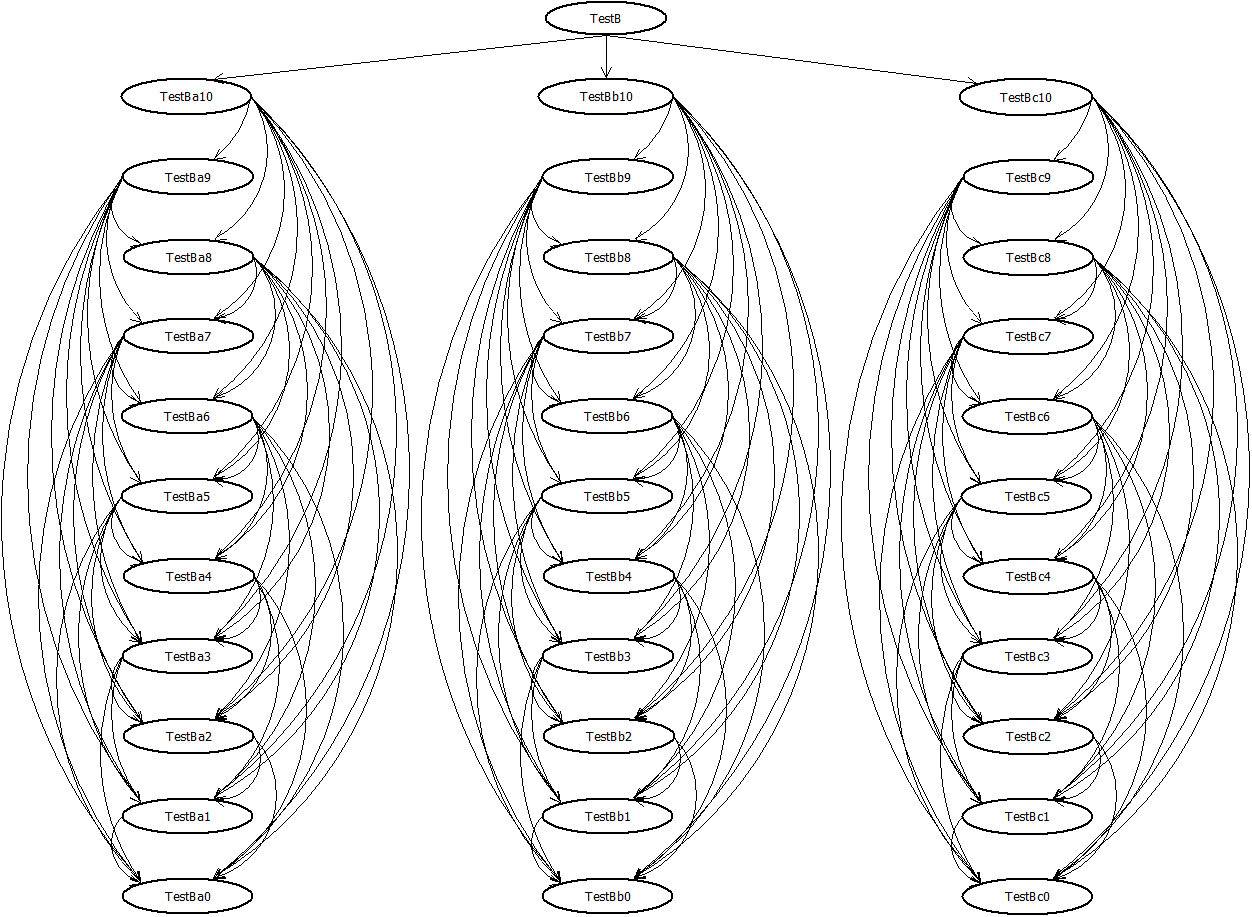
\includegraphics[width=\linewidth]{TestB.png}
  		\caption{Graf zależności dla testu B.}
  		\label{fig:testB}
	\end{center}
\end{figure}\\
Łatwo wywnioskować, że tworząc obiekty poszczególnych typów ilość tworzonych obiektów rośnie dwukrotnie (tak jak dla testu A):
\begin{itemize}
	\item TestBa0 - 1 obiekt,
	\item TestBa1 - 2 obiekty (obiekt typu TestBa1 i obiekt typu TestBa0),
	\item TestBa2 - 4 obiekty (obiekt typu TestBa2, obiekt typu TestBa1 - 2 obiekty, obiekt typu TestBa0 - 1 obiekt),
	\item TestBa3 - 8 obiektów (obiekt typu TestBa3, obiekt typu TestBa2 - 4 obiekty, obiekt typu TestBa1 - 2 obiekty, obiekt typu TestBa0 - 1 obiekt),
	\item TestBa4 - 16 obiektów,
	\item TestBa5 - 32 obiektów,
	\item TestBa6 - 64 obiektów,
	\item TestBa7 - 128 obiektów,
	\item TestBa8 - 256 obiektów,
	\item TestBa9 - 512 obiektów,
	\item TestBa10 - 1 024 obiektów,
	\item \ldots (dla typów od TestBb0 do TestBb10 i od TestBc0 do TestBc10 sytuacja wygląda dokłądnie tak samo jak dla typów od TestBa0 do TestBa10),
	\item TestB - 3 073 obiektów.
\end{itemize}
Zatem tworząc obiekt typu TestB, tworzymy: 1 obiekt typu TestB, 1 obiekt typu TestBa10, TestBb10 i TestBc10, 1 obiekt typu TestBa9, TestBb9 i TestBc9, 2 obiekty typu TestBa8, TestBb8 i TestBc8, 4 obiekty typu TestBa7, TestBb7 i TestBc7, 8 obiektów typu TestBa6, TestBb6 i TestBc6, 16 obiektów typu TestBa5, TestBb5 i TestBc5, 32 obiektów typu TestBa4, TestBb4 i TestBc4, 64 obiektów typu TestBa3, TestBb3 i TestBc3, 128 obiektów typu TestBa2, TestBb2 i TestBc2, 256 obiektów typu TestBa1, TestBb1 i TestBc1, 512 obiektów typu TestBa0, TestBb0 i TestBc0 - co daje w sumie 3 073 obiektów.

\subsubsection{Wyniki dla Singleton}
\begin{center}
\begin{small}
	\begin{tabular}{ | l | r r r | r r r | r r r | r r r | }
    		\hline
Ilość & & 1 & & & 10 & & & 100 & & & 1000 & \\ \hline
 & min & max & avg & min & max & avg & min & max & avg & min & max & avg \\ \hline
Autofac & 0 & 0 & 0 & 0 & 0 & 0 & 0 & 0 & 0 & 0 & 0 & 0 \\ \hline
DryIoc & 8 & 8 & 8 & 8 & 9 & 8 & 8 & 9 & 8 & 8 & 9 & 8 \\ \hline
Grace & 8 & 8 & 8 & 8 & 8 & 8 & 8 & 8 & 8 & 8 & 8 & 8 \\ \hline
LightInject & 6 & 7 & 6 & 6 & 7 & 6 & 6 & 7 & 6 & 6 & 7 & 6 \\ \hline
Ninject & 9 & 10 & 9 & 9 & 10 & 9 & 9 & 11 & 10 & 12 & 13 & 12 \\ \hline
NiquIoCPartial & 4 & 4 & 4 & 4 & 4 & 4 & 4 & 5 & 4 & 4 & 4 & 4 \\ \hline
NiquIoCFull & 8 & 9 & 8 & 8 & 8 & 8 & 8 & 8 & 8 & 8 & 8 & 8 \\ \hline
SimpleInjector & 6 & 6 & 6 & 6 & 6 & 6 & 6 & 6 & 6 & 6 & 6 & 6 \\ \hline
StructureMap & 32 & 33 & 33 & 32 & 33 & 33 & 32 & 34 & 33 & 33 & 34 & 33 \\ \hline
Unity & 23 & 24 & 23 & 23 & 24 & 23 & 23 & 24 & 24 & 24 & 25 & 24 \\ \hline
Windsor & 0 & 0 & 0 & 0 & 0 & 0 & 0 & 0 & 0 & 0 & 0 & 0 \\ \hline
  	\end{tabular}
\end{small}
\end{center}
Podobnie jak dla przypadku testowego A, tutaj również najlepiej poradziły sobie najpopularniejsze rozwiązania - Aurofac i Windsor. Warto zaznaczyć, że to jedyne rozwiązania, które nie zanotowały znaczącego wzrotu czasu. Dla pozostałych rozwiązań czasy wzrosły od 2 do 4 razy. NiquIoCPartial uplasował się tutaj również na 3 miejscu, a za nim SimpleInjector oraz LightInject. Koniec rankingu jest taki sam, czyli Ninject, Unity i StructureMap. NiquIoCFull, Grace, a także DryIoc miały zbliżone do siebie czasy - trochę słabsze niż LightInject i trochę lepsze niż Ninject.

\subsubsection{Wyniki dla Transient}
\begin{center}
\begin{small}
	\begin{tabular}{ | l | r r r | r r r | r r r | r r r | }
    		\hline
Ilość & & 1 & & & 10 & & & 100 & & & 1000 & \\ \hline
 & min & max & avg & min & max & avg & min & max & avg & min & max & avg \\ \hline
Autofac & 2 & 2 & 2 & 21 & 25 & 21 & 189 & 201 & 191 & 1890 & 2044 & 1903 \\ \hline
DryIoc & 43 & 44 & 43 & 44 & 45 & 44 & 51 & 52 & 51 & 97 & 100 & 98 \\ \hline
Grace & 50 & 59 & 51 & 51 & 55 & 52 & 57 & 59 & 58 & 122 & 128 & 124 \\ \hline
LightInject & 31 & 33 & 32 & 32 & 33 & 32 & 37 & 38 & 37 & 70 & 73 & 71 \\ \hline
Ninject & 36 & 38 & 36 & 276 & 337 & 284 & 2733 & 3595 & 2790 & 28220 & 29976 & 28720 \\ \hline
NiquIoCPartial & 5 & 5 & 5 & 10 & 10 & 10 & 59 & 79 & 61 & 543 & 633 & 550 \\ \hline
NiquIoCFull & 26 & 27 & 26 & 26 & 27 & 26 & 32 & 33 & 32 & 66 & 68 & 66 \\ \hline
SimpleInjector & 40 & 41 & 40 & 40 & 42 & 41 & 47 & 48 & 47 & 95 & 97 & 96 \\ \hline
StructureMap & 33 & 34 & 33 & 45 & 46 & 45 & 167 & 175 & 168 & 1333 & 1565 & 1346 \\ \hline
Unity & 28 & 29 & 28 & 49 & 50 & 49 & 260 & 271 & 262 & 2355 & 2419 & 2366 \\ \hline
Windsor & 6 & 7 & 6 & 49 & 69 & 50 & 476 & 610 & 484 & 4726 & 5665 & 4799 \\ \hline
  	\end{tabular}
\end{small}
\end{center}
Dla tego testu sytuacja wygląda niemal identycznie jak w teście A, z tą różnicą, że czasy dla każdego rozwiązania są ponad 3 razy większe.\\
Przy 1 operację najlepiej radzi sobie Autofac, a tuż za nim NiquIoCPartial i Windsor. Pozostałe rozwiązania wypadły słabo i mają czasy od kilku do kilkunastu razy większe niż czołówka. Kolejne miejsca to: NiquIocFull, Unity, LightInject, StructureMap oraz Ninject, a ranking zamykają SimplyInjector, DryIoc i Grace.\\
Gdy mamy 10 operacji najlepiej radzi sobie NiquIoCPartial, a zaraz za nim z czasem dwókrotnie gorszym jest Autofac. Następnie w rankingu znajduje się NiquIoCFull i LightInject. Tutaj również jak w przypadku testowym A, Ninject ma ponad 5 razy gorszy czas niż miejsce przedostatnie, z tą różnicą, że zajmuje je Grace, a nie Windsor, który uzyskał trochę lepszy czas i jest miejsce wyżej. Lepiej od Windsor poradziły sobie jeszcze: SimpleInjector, DryIoc, StructureMap i Unity, ale do czołówki brakowało im bardzo dużo.\\
Dla 100 operacji nic się nie zmieniło w stosunku do testu A. Pierwsze trzy miejsca zajmują: NiquIoCFull, LightInject i SimpleInjector. Grace z miejsca przedostatniego dla 10 operacji, awansował na miejsce piąte. Przed nim znalazł się DryIoc, a tuż za nim NiquIoCPartial. Czas całej trójki są zadowalające. Grono najsłabszych to: StructureMap, Autofac, Unity, Windsor i Ninject.\\
Jak można się było spodziewać przy 1000 operacji sytuacja wygląda identycznie - pod względem czasu od czołówki oddalił się NiquIoCPartial, a na pierwszym miejscu wciąż pozostaje NiquIoCFull. LightInject oraz SimpleInjector są kawałek za nim. Dalej DryIoc i Grace wciąż akceptowalnie. Miejsce w środku rankingu zajmuje NiquIoCPartial, a pozostałe rozwiązania mają od niego o rząd lub dwa większe czasy.\\
Tutaj również najmniejszy wzorst czasów miały rozwiązania: LightInject, NiquIoCFull, SimpleInjector, DryIoc oraz Grace.

\subsubsection{Wyniki dla TransientSingleton}
\begin{center}
\begin{small}
	\begin{tabular}{ | l | r r r | r r r | r r r | r r r | }
    		\hline
Ilość & & 1 & & & 10 & & & 100 & & & 1000 & \\ \hline
 & min & max & avg & min & max & avg & min & max & avg & min & max & avg \\ \hline
Autofac & 1 & 2 & 1 & 18 & 20 & 18 & 172 & 206 & 173 & 1698 & 1832 & 1709 \\ \hline
DryIoc & 56 & 57 & 56 & 57 & 58 & 57 & 64 & 65 & 64 & 108 & 110 & 109 \\ \hline
Grace & 30 & 32 & 31 & 31 & 32 & 31 & 35 & 37 & 35 & 69 & 72 & 69 \\ \hline
LightInject & 48 & 50 & 48 & 48 & 50 & 48 & 51 & 53 & 51 & 80 & 82 & 80 \\ \hline
Ninject & 29 & 34 & 30 & 214 & 239 & 219 & 2013 & 2426 & 2063 & 20440 & 22891 & 20858 \\ \hline
NiquIoCPartial & 4 & 5 & 5 & 8 & 9 & 8 & 41 & 57 & 42 & 365 & 406 & 368 \\ \hline
NiquIoCFull & 16 & 16 & 16 & 16 & 17 & 16 & 18 & 19 & 18 & 37 & 39 & 38 \\ \hline
SimpleInjector & 28 & 28 & 28 & 28 & 29 & 28 & 32 & 34 & 32 & 61 & 62 & 61 \\ \hline
StructureMap & 33 & 34 & 33 & 40 & 46 & 40 & 112 & 123 & 113 & 797 & 915 & 805 \\ \hline
Unity & 27 & 28 & 27 & 46 & 47 & 46 & 226 & 263 & 228 & 2016 & 2305 & 2032 \\ \hline
Windsor & 3 & 5 & 3 & 37 & 46 & 37 & 355 & 435 & 362 & 3543 & 4824 & 3637 \\ \hline
  	\end{tabular}
\end{small}
\end{center}
Jeśli chodzi o wzrost czasów w stosnku do przypadku testowego A, to sytuacja wygląda niemal identycznie jak dla testu Transient - jest on ponad trzykrotny.\\
Dla 1 operacji podium wygląda jednak inaczej niż dla testu A - miejscami zamieniły się NiquIocPartial i Windsor. Na pierwszy miejscu pozostaje Autofac. Różnice czasów dla pozostałych rozwiązań są już dużo bardziej zauważalne. Znajdujący się tuż za podium NiquIoCFull ma wynik ponad trzy razy słabszy niż NiquIoCPartial, który to podium zamyka. Kolejne miejsca to: Unity, SimpleInjector, Ninject, Grace, StructureMap, Lightinject i na końcu DryIoc.\\
Gry mamy 10 operacji pierwsze dwa miejsca zajmują NiquIoCPartial i NiquIoCFull. Tuż za nimi znajduje się Autofac. SimplyInjector oraz Grace zanotowały niewielki wzrost czasów i zajmują kolejne dwa miejsca. Nieduży wzrostu czasów zaliczyły również LightInject i DryIoc, ale ich czasy są wciąż duże w stosunku do pozostałych rozwiążań i zajmuje dwa przedostatnie miejsca - ustępując jedynie Ninject. Miejsca od 6 do 8 przypadły: Windsor, StructureMap oraz Unity.\\
Przy 100 i 1000 operacjach nie ma już żadnych zmian w rankingu względem testu A.\\
Dla pierwszego przypadku początek rankingu wygląda następująco: NiquIocFull, SimpleInjector i Grace. Zaraz za podium znajduje się NiquIocPartial. LightInject oraz DryIoc dzięki niedużemu wzrostowi czasów znalazły się na miejscach piątym i szóstym. Są to ostatnie zadowalające rozwiązania. Kolejne miejsca zajmują: StrucutreMap, Autofac, Unity, Windsor oraz Ninject.\\
Dla drugiego przypadku pierwsze trzy miejsca są jak wyżej. Natomiast o jedno miejsce awansowały LightInject oraz Grace. NiquIoCPartial spadł na miejsce szóste i dołączył do grupy rozwiązań z bardzo dużymi czasami. Reszta rankingu nie uległa zmianie.

\subsubsection{Wyniki dla PerThread}
\begin{center}
\begin{small}
	\begin{tabular}{ | l | r r r | r r r | r r r | r r r | }
    		\hline
Ilość & & 1 & & & 10 & & & 100 & & & 1000 & \\ \hline
 & min & max & avg & min & max & avg & min & max & avg & min & max & avg \\ \hline
Autofac & 0 & 0 & 0 & 0 & 0 & 0 & 0 & 0 & 0 & 0 & 0 & 0 \\ \hline
DryIoc & 246 & 250 & 247 & 246 & 250 & 247 & 246 & 248 & 247 & 246 & 249 & 247 \\ \hline
Grace & 13 & 13 & 13 & 13 & 13 & 13 & 13 & 14 & 13 & 13 & 14 & 13 \\ \hline
LightInject & 409 & 419 & 412 & 409 & 432 & 413 & 409 & 416 & 412 & 409 & 420 & 413 \\ \hline
Ninject & 9 & 10 & 9 & 9 & 10 & 9 & 9 & 10 & 10 & 12 & 13 & 13 \\ \hline
NiquIoCPartial & 4 & 5 & 4 & 4 & 4 & 4 & 4 & 4 & 4 & 4 & 5 & 4 \\ \hline
NiquIoCFull & 8 & 8 & 8 & 8 & 8 & 8 & 8 & 8 & 8 & 8 & 8 & 8 \\ \hline
SimpleInjector & 23 & 23 & 23 & 23 & 23 & 23 & 23 & 23 & 23 & 23 & 24 & 23 \\ \hline
StructureMap & 32 & 34 & 33 & 32 & 38 & 33 & 33 & 35 & 33 & 33 & 34 & 33 \\ \hline
Unity & 23 & 25 & 23 & 23 & 24 & 23 & 23 & 24 & 23 & 24 & 25 & 24 \\ \hline
Windsor & 0 & 0 & 0 & 0 & 0 & 0 & 0 & 0 & 0 & 0 & 0 & 0 \\ \hline
  	\end{tabular}
\end{small}
\end{center}
Podobnie jak było dla przypadku testowego A, tutaj również nie wszystkie rozwiązania mają czasy zbliżone do Singleton.\\
Są to te same rozwiązania co dla testu A, czyli: SimpleInjector, DryIoc i LightInject. Warto jednak zaznaczyć, że dla SimpleInjector wzrost czasów jest kilkukrotny, a dla pozostałych dwóch rozwiązań kilkudziesięciokrotny.\\
Tak samo jak w przypadku Signleton czołówka wygląda następująco: Aurofac, Windsor i NiquIoCPartial. Kolejne miejsca zajmują: NiquIoCFull, Ninject i Grace. Najsłabiej poradziły sobie rozwiążania LightInject i DryIoc. W środku tabeli pod względem czasów znalazły się SimpleInjector, Unity i StrucutreMap. W odróżnieniu od przypadku testowego A, tutaj nie było żadnych zmian w rankingu i wszystkie rozwiązania zajmują te same miejsca dla dowolnej liczby operacji.


\subsection{Przypadek testowy C}
\subsubsection{Opis}
W tym teście mamy zdefiniowanych 26 typów. 5 z tych typów ma konstruktor bezparametrowy, a pozostałe 21 ma konstuktor z pięcioma parametrami. Typem głównym jest typ "TestC". Obiekt tego typy w konstruktorze przymuje 5 innych obiektów, kolejno następujących typów: "TestC40", "TestC41", "TestC42", "TestC43" i "TestC44". Każdy z tych pięciu typów ma taki sam konstruktor - przyjmuje w nim 5 obiektów o typach z pierwszym numerkiem o 1 mniejszym (czyli przyjmują w konstruktorze obiekty typów od "TestC30" do "TestC34"). Dla typów od "TestC30" do "TestC34" zasad z konstruktorami wygląda tak samo. Na końcu dochodzimy do typów od "TestC00" do "TestC04", które mają konstruktor bezparametrowy. Rys. \ref{fig:testC} przedstawia graf zależności typów dla tego przypadku testowego.

\begin{figure}[h]
	\begin{center}
  		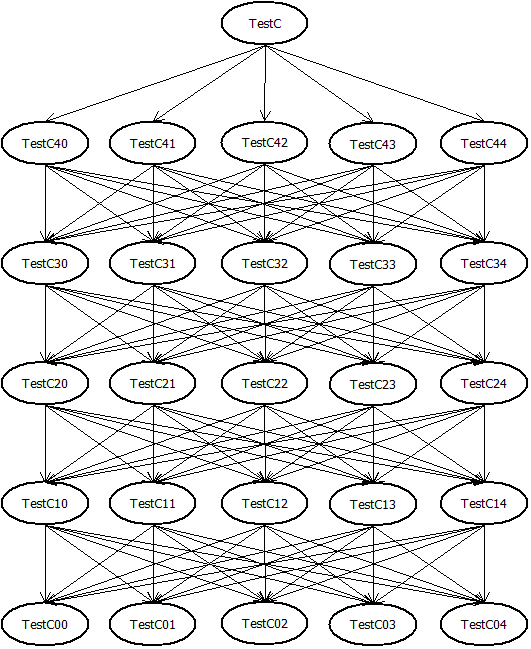
\includegraphics[height=10cm]{TestC.png}
  		\caption{Graf zależności dla testu C.}
  		\label{fig:testC}
	\end{center}
\end{figure}

Łatwo wywnioskować, że tworząc obiekty poszczególnych typów ilość tworzonych obiektów rośnie ponad dziesięciokortnie:
\begin{itemize}
	\item typy od TestC00 do TestC04 - 1 obiekt,
	\item typy od TestC10 do TestC14 - 6 obiektów (obiekt danego typu plus 5 obiektów typów od TestC00 do TestC04),
	\item typy od TestC20 do TestC24 - 31 obiektów (obiekt danego typu plus 5 obiektów typów od TestC10 do TestC14),
	\item typy od TestC30 do TestC34 - 156 obiektów,
	\item  typy od TestC40 do TestC44 - 781 obiektów,
	\item TestC - 3 906 obiektów.
\end{itemize}
Zatem tworząc obiekt typu TestC, tworzymy: 1 obiekt typu TestC, 5 obiektów typów od TestC40 do TestC44, 25 obiektów typów od TestC30 do TestC34, 125 obiektów typów od TestC20 do TestC24, 625 obiektów typów od TestC10 do TestC14, 3 125 obiektów typów od TestC00 do TestC04 - co daje w sumie 3 906 obiektów.

\subsubsection{Wyniki dla Singleton}
\begin{center}
\begin{small}
	\begin{tabular}{ | l | r r r | r r r | r r r | r r r | }
    		\hline
Ilość & & 1 & & & 10 & & & 100 & & & 1000 & \\ \hline
 & min & max & avg & min & max & avg & min & max & avg & min & max & avg \\ \hline
Autofac & 0 & 0 & 0 & 0 & 0 & 0 & 0 & 0 & 0 & 0 & 0 & 0 \\ \hline
DryIoc & 5 & 5 & 5 & 5 & 5 & 5 & 5 & 5 & 5 & 5 & 5 & 5 \\ \hline
Grace & 5 & 5 & 5 & 5 & 5 & 5 & 5 & 5 & 5 & 5 & 5 & 5 \\ \hline
LightInject & 4 & 4 & 4 & 4 & 4 & 4 & 4 & 4 & 4 & 4 & 4 & 4 \\ \hline
Ninject & 6 & 6 & 6 & 6 & 6 & 6 & 6 & 7 & 6 & 9 & 10 & 9 \\ \hline
NiquIoCPartial & 3 & 3 & 3 & 3 & 3 & 3 & 3 & 3 & 3 & 3 & 3 & 3 \\ \hline
NiquIoCFull & 5 & 5 & 5 & 5 & 5 & 5 & 5 & 5 & 5 & 5 & 5 & 5 \\ \hline
SimpleInjector & 4 & 4 & 4 & 4 & 4 & 4 & 4 & 4 & 4 & 4 & 4 & 4 \\ \hline
StructureMap & 22 & 23 & 22 & 22 & 23 & 22 & 22 & 23 & 22 & 23 & 24 & 23 \\ \hline
Unity & 15 & 16 & 15 & 15 & 16 & 15 & 15 & 16 & 15 & 16 & 17 & 16 \\ \hline
Windsor & 0 & 0 & 0 & 0 & 0 & 0 & 0 & 0 & 0 & 0 & 0 & 0 \\ \hline
  	\end{tabular}
\end{small}
\end{center}
<<opis>>

\subsubsection{Wyniki dla Transient}
\begin{center}
\begin{small}
	\begin{tabular}{ | l | r r r | r r r | r r r | r r r | }
    		\hline
Ilość & & 1 & & & 10 & & & 100 & & & 1000 & \\ \hline
 & min & max & avg & min & max & avg & min & max & avg & min & max & avg \\ \hline
Autofac & 2 & 2 & 2 & 23 & 25 & 24 & 229 & 250 & 231 & 2274 & 2419 & 2288 \\ \hline
DryIoc & 39 & 41 & 39 & 40 & 41 & 40 & 47 & 48 & 47 & 98 & 100 & 99 \\ \hline
Grace & 61 & 63 & 61 & 62 & 65 & 62 & 73 & 74 & 73 & 153 & 163 & 155 \\ \hline
LightInject & 36 & 37 & 36 & 36 & 39 & 37 & 43 & 49 & 44 & 86 & 88 & 86 \\ \hline
Ninject & 38 & 42 & 39 & 345 & 375 & 353 & 3430 & 4043 & 3511 & 36072 & 42914 & 37642 \\ \hline
NiquIoCPartial & 3 & 4 & 4 & 10 & 11 & 10 & 72 & 80 & 74 & 683 & 781 & 690 \\ \hline
NiquIoCFull & 31 & 33 & 31 & 31 & 33 & 32 & 38 & 41 & 38 & 81 & 83 & 82 \\ \hline
SimpleInjector & 40 & 42 & 41 & 41 & 43 & 41 & 49 & 51 & 49 & 115 & 117 & 116 \\ \hline
StructureMap & 26 & 27 & 26 & 40 & 42 & 40 & 178 & 207 & 181 & 1520 & 1810 & 1540 \\ \hline
Unity & 18 & 19 & 19 & 47 & 51 & 47 & 315 & 369 & 318 & 2995 & 3359 & 3015 \\ \hline
Windsor & 7 & 8 & 7 & 61 & 82 & 62 & 594 & 769 & 608 & 5898 & 7708 & 6037 \\ \hline
  	\end{tabular}
\end{small}
\end{center}
<<opis>>

\subsubsection{Wyniki dla TransientSingleton}
\begin{center}
\begin{small}
	\begin{tabular}{ | l | r r r | r r r | r r r | r r r | }
    		\hline
Ilość & & 1 & & & 10 & & & 100 & & & 1000 & \\ \hline
 & min & max & avg & min & max & avg & min & max & avg & min & max & avg \\ \hline
Autofac & 1 & 2 & 2 & 19 & 20 & 20 & 184 & 198 & 187 & 1810 & 1898 & 1831 \\ \hline
DryIoc & 58 & 70 & 58 & 59 & 62 & 59 & 65 & 68 & 65 & 105 & 107 & 106 \\ \hline
Grace & 23 & 24 & 23 & 23 & 24 & 23 & 25 & 26 & 25 & 44 & 45 & 44 \\ \hline
LightInject & 52 & 54 & 52 & 52 & 55 & 53 & 55 & 57 & 56 & 82 & 85 & 83 \\ \hline
Ninject & 25 & 30 & 26 & 199 & 231 & 203 & 1903 & 2364 & 1951 & 19137 & 22595 & 19626 \\ \hline
NiquIoCPartial & 3 & 3 & 3 & 6 & 7 & 6 & 38 & 46 & 39 & 347 & 359 & 349 \\ \hline
NiquIoCFull & 12 & 13 & 12 & 12 & 13 & 12 & 13 & 14 & 14 & 25 & 26 & 25 \\ \hline
SimpleInjector & 21 & 22 & 21 & 21 & 22 & 21 & 23 & 24 & 24 & 44 & 45 & 44 \\ \hline
StructureMap & 23 & 23 & 23 & 30 & 31 & 30 & 80 & 84 & 80 & 549 & 593 & 553 \\ \hline
Unity & 18 & 18 & 18 & 39 & 41 & 40 & 242 & 258 & 243 & 2258 & 2428 & 2272 \\ \hline
Windsor & 3 & 3 & 3 & 34 & 41 & 35 & 338 & 400 & 343 & 3368 & 4115 & 3429 \\ \hline
  	\end{tabular}
\end{small}
\end{center}
<<opis>>

\subsubsection{Wyniki dla PerThread}
\begin{center}
\begin{small}
	\begin{tabular}{ | l | r r r | r r r | r r r | r r r | }
    		\hline
Ilość & & 1 & & & 10 & & & 100 & & & 1000 & \\ \hline
 & min & max & avg & min & max & avg & min & max & avg & min & max & avg \\ \hline
Autofac & 0 & 0 & 0 & 0 & 0 & 0 & 0 & 0 & 0 & 0 & 0 & 0 \\ \hline
DryIoc & 157 & 162 & 158 & 157 & 160 & 158 & 157 & 160 & 158 & 158 & 161 & 158 \\ \hline
Grace & 8 & 9 & 8 & 8 & 9 & 8 & 8 & 9 & 8 & 8 & 9 & 8 \\ \hline
LightInject & 525 & 556 & 529 & 525 & 551 & 530 & 525 & 558 & 530 & 525 & 550 & 529 \\ \hline
Ninject & 6 & 7 & 6 & 6 & 6 & 6 & 6 & 7 & 6 & 9 & 10 & 9 \\ \hline
NiquIoCPartial & 3 & 3 & 3 & 3 & 3 & 3 & 3 & 3 & 3 & 3 & 3 & 3 \\ \hline
NiquIoCFull & 5 & 5 & 5 & 5 & 5 & 5 & 5 & 5 & 5 & 5 & 5 & 5 \\ \hline
SimpleInjector & 16 & 16 & 16 & 16 & 16 & 16 & 16 & 16 & 16 & 16 & 18 & 16 \\ \hline
StructureMap & 22 & 23 & 22 & 22 & 23 & 22 & 22 & 23 & 22 & 23 & 73 & 24 \\ \hline
Unity & 15 & 16 & 15 & 15 & 16 & 15 & 15 & 16 & 15 & 16 & 17 & 16 \\ \hline
Windsor & 0 & 0 & 0 & 0 & 0 & 0 & 0 & 0 & 0 & 0 & 0 & 0 \\ \hline
  	\end{tabular}
\end{small}
\end{center}
<<opis>>


\subsection{Przypadek testowy D}
\subsubsection{Opis}
W tym teście mamy zdefiniowanych 51 typów. 10 z tych typów ma konstruktor bezparametrowy, a pozostałe 41 ma konstuktor z dziesięcioma parametrami. Typem głównym jest typ "TestD". Obiekt tego typy w konstruktorze przymuje 10 innych obiektów, kolejno następujących typów: "TestD40", "TestD41", "TestD42", "TestD43", "TestD44", "TestD45", "TestD46", "TestD47", "TestD48", "TestD49". Każdy z tych 10 typów w konstruktorze przyjmuje 10 obiektów o takich samych typach, ale z pierwszym numerkiem o 1 mniejszym (czyli obiekty typów od "TestD40" do "TestD49", przyjmują w konstruktorze obiekty typów od "TestD30" do "TestD39"). Dla typów od "TestD30" do "TestD39" zasad z konstruktorami wygląda tak samo. Na końcu dochodzimy do typów od "TestD00" do "TestD09", które mają konstruktor bezparametrowy. Rys. \ref{fig:testD} przedstawia graf zależności typów dla tego przypadku testowego.

\begin{figure}[h]
	\begin{center}
  		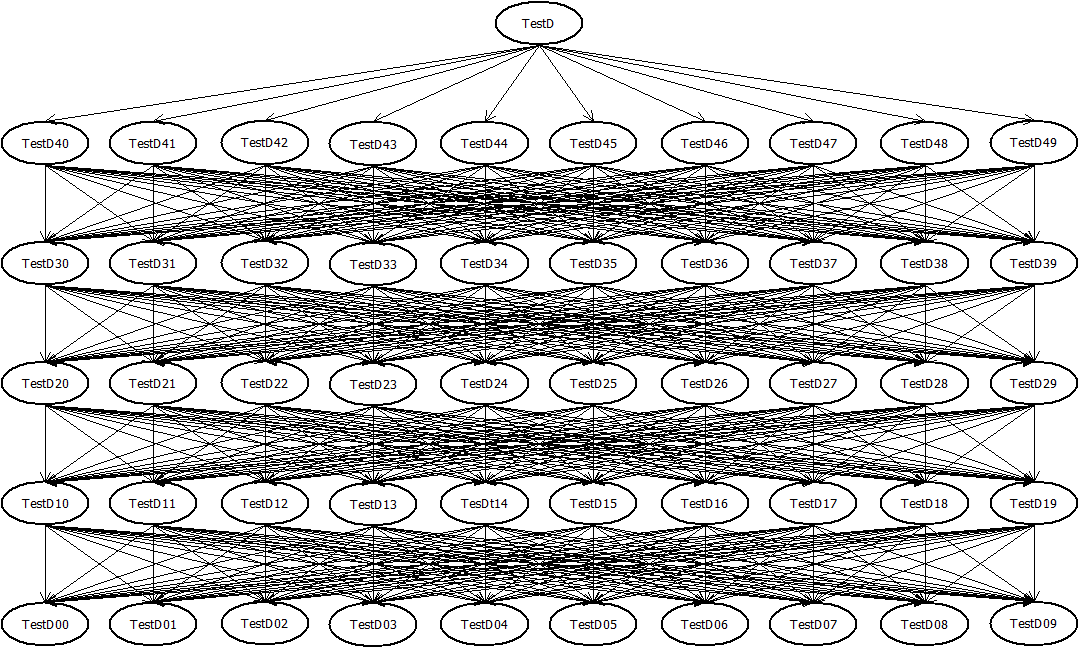
\includegraphics[width=\linewidth]{TestD.png}
  		\caption{Graf zależności dla testu D.}
  		\label{fig:testD}
	\end{center}
\end{figure}

Łatwo wywnioskować, że tworząc obiekty poszczególnych typów ilość tworzonych obiektów rośnie ponad dziesięciokortnie:
\begin{itemize}
	\item typy od TestD00 do TestD09 - 1 obiekt,
	\item typy od TestD10 do TestD19 - 11 obiektów (obiekt danego typu plus 10 obiektów typów od TestD00 do TestD09),
	\item typy od TestD20 do TestD29 - 111 obiektów (obiekt danego typu plus 10 obiektów typów od TestD10 do TestD19),
	\item typy od TestD30 do TestD39 - 1 111 obiektów,
	\item  typy od TestD40 do TestD49 - 11 111 obiektów,
	\item TestD - 111 111 obiektów.
\end{itemize}
Zatem tworząc obiekt typu TestD, tworzymy: 1 obiekt typu TestD, 10 obiektów typów od TestD40 do TestD49, 100 obiektów typów od TestD30 do TestD39, 1 000 obiektów typów od TestD20 do TestD29, 10 000 obiektów typów od TestD10 do TestD19, 100 000 obiektów typów od TestD00 do TestD09 - co daje w sumie 111 111 obiektów..

\subsubsection{Wyniki dla Singleton}
\begin{center}
\begin{small}
	\begin{tabular}{ | l | r r r | r r r | }
    		\hline
Ilość & & 1 & & & 10 & \\ \hline
 & min & max & avg & min & max & avg \\ \hline
Autofac & 0 & 0 & 0 & 0 & 0 & 0 \\ \hline
DryIoc & 10 & 10 & 10 & 10 & 10 & 10 \\ \hline
Grace & 16 & 17 & 16 & 16 & 17 & 16 \\ \hline
LightInject & 14 & 14 & 14 & 14 & 15 & 14 \\ \hline
Ninject & 21 & 22 & 21 & 21 & 22 & 21 \\ \hline
NiquIoCPartial & 8 & 9 & 9 & 8 & 9 & 8 \\ \hline
NiquIoCFull & 18 & 19 & 18 & 18 & 19 & 18 \\ \hline
SimpleInjector & 11 & 12 & 11 & 11 & 12 & 11 \\ \hline
StructureMap & 49 & 50 & 49 & 49 & 50 & 49 \\ \hline
Unity & 52 & 53 & 52 & 52 & 54 & 52 \\ \hline
Windsor & 0 & 0 & 0 & 0 & 0 & 0 \\ \hline
  	\end{tabular}
\end{small}
\end{center}
Podobnie jak dla przypadku testowego A, tutaj również najlepiej poradziły sobie najpopularniejsze rozwiązania - Windsor i Aurofac. Na trzecim miejscu znajduje się rozwiązanie NiquIoCPartial. Najsłabiej poradził sobie rozwiązania StructureMap i Unity.

\subsubsection{Wyniki dla Transient}
\begin{center}
\begin{small}
	\begin{tabular}{ | l | r r r | r r r | }
    		\hline
Ilość & & 1 & & & 10 & \\ \hline
 & min & max & avg & min & max & avg \\ \hline
Autofac & 136 & 160 & 147 & 1161 & 1279 & 1188 \\ \hline
DryIoc & 979 & 996 & 982 & 1013 & 1025 & 1015 \\ \hline
Grace & 1413 & 1472 & 1426 & 1465 & 1558 & 1495 \\ \hline
LightInject & 797 & 831 & 812 & 841 & 878 & 853 \\ \hline
Ninject & 1016 & 1179 & 1039 & 10072 & 11599 & 10307 \\ \hline
NiquIoCPartial & 36 & 38 & 37 & 285 & 291 & 287 \\ \hline
NiquIoCFull & 566 & 576 & 569 & 619 & 661 & 631 \\ \hline
SimpleInjector & 177 & 179 & 178 & 205 & 212 & 206 \\ \hline
StructureMap & 102 & 110 & 103 & 586 & 603 & 591 \\ \hline
Unity & 150 & 200 & 152 & 1073 & 1183 & 1080 \\ \hline
Windsor & 177 & 261 & 182 & 1797 & 2421 & 1827 \\ \hline
  	\end{tabular}
\end{small}
\end{center}
Dla tego testu rozbierzność czasów jest dość duża.\\
Gdy mamy tylko 1 operację najlepiej radzi sobie NiquIoCPartial. Czasy pozostały są znacząco większe. Najsłabiej poradziły sobie Grace, Ninject, DryIoc i LightInject.\\
Dla 10 operacji znacząco najlepiej radzi sobie SimplyInjector i NiquIoCPartial. Czołówkę zamykają StrucutreMap i NiquIoCFull. Pozostałe rozwiązania miały podobne, dużo słabsze czasy. Wyjątkiem jest ponownie Ninject, którego czasy są kilkukrotnie większe.\\
W tym przypadku najmniejszy wzorst czasu miały kolejno rozwiązania: DryIoc, SimpleInjector, LightInject, Grace oraz NiquIoCFull.

\subsubsection{Wyniki dla TransientSingleton}
\begin{center}
\begin{small}
	\begin{tabular}{ | l | r r r | r r r | }
    		\hline
Ilość & & 1 & & & 10 & \\ \hline
 & min & max & avg & min & max & avg \\ \hline
Autofac & 77 & 84 & 78 & 893 & 964 & 910 \\ \hline
DryIoc & 905 & 922 & 910 & 936 & 983 & 942 \\ \hline
Grace & 374 & 386 & 376 & 381 & 396 & 383 \\ \hline
LightInject & 1285 & 1358 & 1310 & 1297 & 1360 & 1316 \\ \hline
Ninject & 503 & 572 & 511 & 4732 & 5620 & 4818 \\ \hline
NiquIoCPartial & 17 & 18 & 17 & 100 & 104 & 101 \\ \hline
NiquIoCFull & 144 & 151 & 145 & 151 & 159 & 152 \\ \hline
SimpleInjector & 85 & 87 & 86 & 91 & 93 & 91 \\ \hline
StructureMap & 60 & 69 & 61 & 165 & 173 & 167 \\ \hline
Unity & 115 & 140 & 116 & 683 & 771 & 689 \\ \hline
Windsor & 85 & 102 & 87 & 852 & 965 & 864 \\ \hline
  	\end{tabular}
\end{small}
\end{center}
<<opis>>

\subsubsection{Wyniki dla PerThread}
\begin{center}
\begin{small}
	\begin{tabular}{ | l | r r r | r r r | }
    		\hline
Ilość & & 1 & & & 10 & \\ \hline
 & min & max & avg & min & max & avg \\ \hline
Autofac & 0 & 0 & 0 & 0 & 0 & 0 \\ \hline
DryIoc & 1042 & 1051 & 1045 & 1042 & 1051 & 1044 \\ \hline
Grace & 28 & 28 & 28 & 28 & 28 & 28 \\ \hline
LightInject & -1 & -1 & -1 & -1 & -1 & -1 \\ \hline
Ninject & 21 & 22 & 21 & 21 & 22 & 21 \\ \hline
NiquIoCPartial & 8 & 9 & 9 & 8 & 10 & 9 \\ \hline
NiquIoCFull & 18 & 18 & 18 & 18 & 18 & 18 \\ \hline
SimpleInjector & 46 & 48 & 46 & 46 & 48 & 46 \\ \hline
StructureMap & 49 & 51 & 49 & 49 & 51 & 49 \\ \hline
Unity & 52 & 53 & 52 & 52 & 53 & 52 \\ \hline
Windsor & 0 & 0 & 0 & 0 & 0 & 0 \\ \hline
  	\end{tabular}
\end{small}
\end{center}
Tutaj tak samo jak dla przypadku testowego A czasy powinny być zbliżone do czasów dla Singleton. Niestety dla tego testu również nie wszystkie rozwiązania sobie z tym poradziły. Dużo słabsze czasy niż w przypadku Singleton miały rozwiązania: DryIoc, Grace, LightInject, SimpleInjector.\\
Zarówno dla 1 jak i 10 powtórzeń najlepiej radzi sobie Autofac i Windsor. Podium ponownie zamyka NiquIoCPartial.\\
Najgorzej poradził sobie tutaj LightInject, który trwał ponad 20 minut (stąd w rozwiążaniu czas "-1"). DryIoc również poradził sobie bardzo słabo - czasy ponad 20 raz gorsze niż rozwiążanie na miejscu o 1 wyższym (Unity).


\clearpage

\section{Podsumowanie}
<parę słów na koniec>

\newpage
\begin{thebibliography}{authordate1}
\bibitem{dependency_injection} Mark Seemann, Dependency Injection in .NET, 2012
\bibitem{emit} Serge Lidin, Expert .NET 2.0 IL Assembler, 2006
\end{thebibliography}

\end{document}